\documentclass{beamer}
\usepackage{../../shared/styles/custom}


%\beamerdefaultoverlayspecification{<+->}
% \newcommand{\data}{\mathcal{D}}
% \newcommand\Item[1][]{%
%   \ifx\relax#1\relax  \item \else \item[#1] \fi
%   \abovedisplayskip=0pt\abovedisplayshortskip=0pt~\vspace*{-\baselineskip}}

\newcommand*{\Comb}[2]{{}^{#1}C_{#2}}%

\graphicspath{ {../assets/ensemble/figures/} }




\title{Ensemble Learning}
\date{\today}
\author{Nipun Batra and teaching staff}
\institute{IIT Gandhinagar}
\begin{document}
\maketitle

\begin{frame}{Ensemble Methods}
  \only<1->{
    Use multiple models for prediction.\\
    Most winning entries of Kaggle competition using ensemble learning.\\
    \vspace{1cm}
  }
  \only<2>{
    \textbf{ Example:}\\
    Classifier 1 - Good\\
    Classifier 2 - Good\\
    Classifier 3 - Bad\\
    \vspace{0.5cm}
    Using Majority Voting, we predict Good.\\
  }
  \only<3>{
    \textbf{ Example:}\\
    Regressor 1 - 20\\
    Regressor 2 - 30\\
    Regressor 3 - 30\\
    \vspace{0.5cm}
    Using Average, we predict $\dfrac{80}{3}$
  }
\end{frame}


\begin{frame}{Intuition}
  \pause Based on \hyperlink{https://web.engr.oregonstate.edu/~tgd/publications/mcs-ensembles.pdf}{Ensemble methods in ML by Dietterich}

  Three reasons why ensembles make sense:

  \pause 1) Statistical: Sometimes if \textbf{data is less, many competing hypothesis can be learnt} all giving same accuracy on training data.

  \pause Eg. We can learn many decision trees for the same data giving same accuracy.

  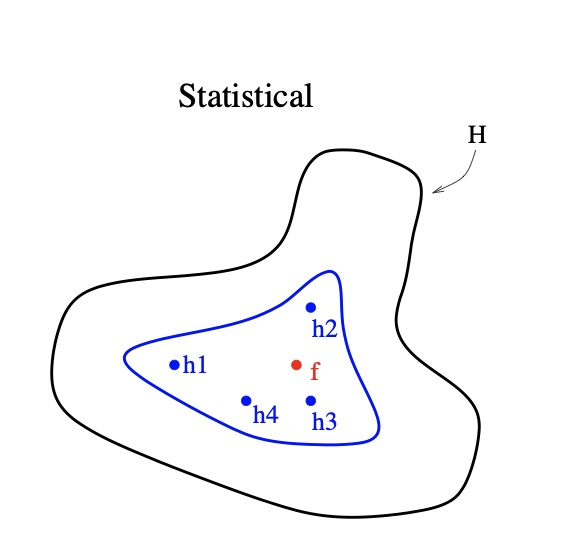
\includegraphics[scale=0.2]{../assets/ensemble/diagrams/statistical.jpg}

\end{frame}
  
\begin{frame}{Intuition}

  \pause 2) Computational: Even if data is enough, some \textbf{classifiers/regressors can get stuck in local optima/apply greedy strategies}. Computationally learning the ``best'' hypothesis can be non-trivial.

  \pause Eg. Decision Trees employ greedy critera

  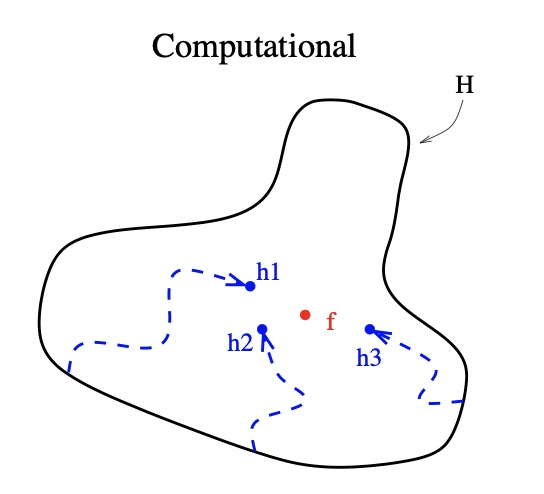
\includegraphics[scale=0.2]{../assets/ensemble/diagrams/computational.jpg}

\end{frame}
  

\begin{frame}{Intuition}

  \pause 3) Representational: Some \textbf{classifiers/regressors can not learn the true form/representation.}

  \pause Eg. Decision Trees can only learn axis-parallel splits.

  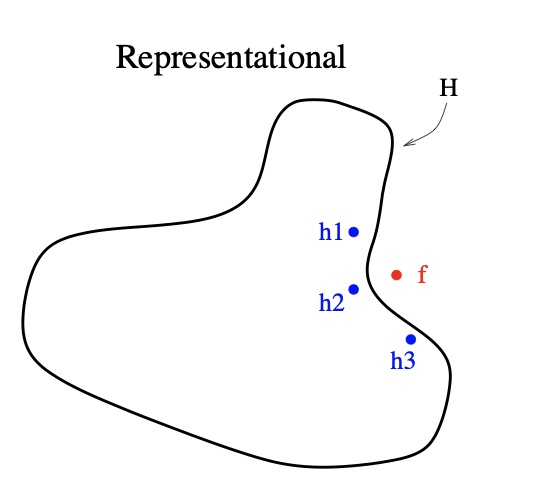
\includegraphics[scale=0.2]{../assets/ensemble/diagrams/representational.jpg}


\end{frame}

\begin{frame}{Representation of Limited Depth DTs vs RFs}

\begin{figure}[htp]
  \centering
  \begin{notebookbox}{https://nipunbatra.github.io/ml-teaching/notebooks/ensemble-representation.html}
    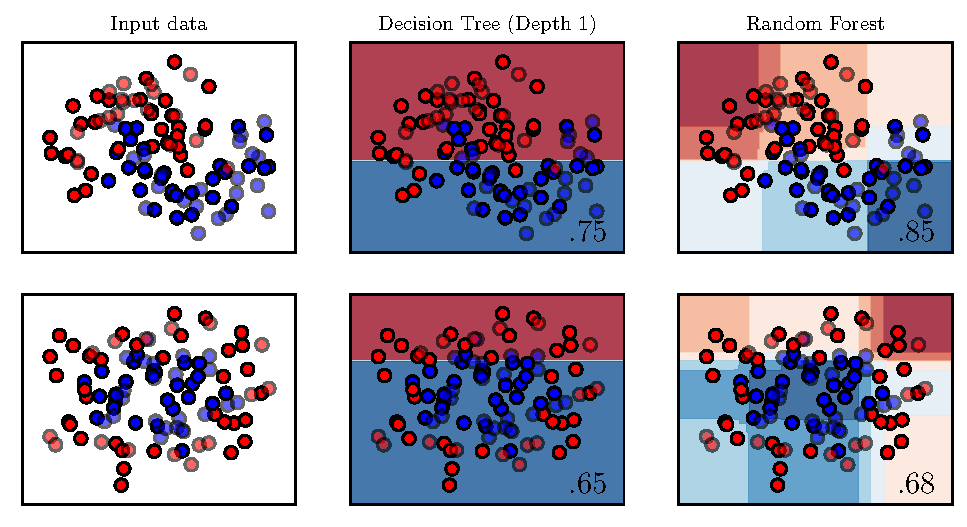
\includegraphics[scale=0.6]{../assets/ensemble/figures/1-representation.pdf}
  \end{notebookbox}
\end{figure}

\end{frame}
\begin{frame}{Representation of Limited Depth DTs vs RFs}

  \begin{figure}[htp]
    \centering
    \begin{notebookbox}{https://nipunbatra.github.io/ml-teaching/notebooks/ensemble-representation.html}
      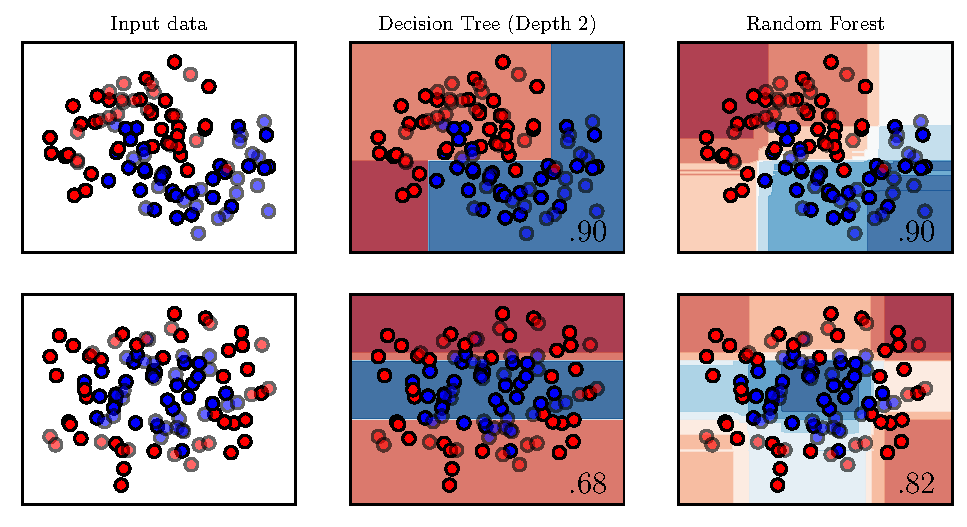
\includegraphics[scale=0.6]{../assets/ensemble/figures/2-representation.pdf}
    \end{notebookbox}
  \end{figure}
  
  \end{frame}




\begin{frame}{Necessary and Sufficient Conditions}
  \pause 1) A necessary and sufficient condition for an ensemble of classifiers to be more
  accurate than any of its individual members is if the classifiers are accurate and
  diverse.

  \pause 2) An accurate classifer: \pause  is one that has an
  error rate of better than random guessing on new x values.

  \pause 3) Two classifiers are diverse: \pause  if they make different errors on new data points

\end{frame}

\begin{frame}{Necessary and Sufficient Conditions}
  Imagine that we have an ensemble of three classifiers ($h_1, h_2, h_3$) and consider a new case x.


  \pause If the three classifiers are identical, i.e.
  not diverse, then when $h_1(x)$ is wrong $h_2(x)$ and $h_3(x)$ will also be wrong.


  \pause However, if the errors made by the classifiers are uncorrelated, then when $h_1(x)$
  is wrong, $h_2(x)$ and $h_3(x)$ may be correct, so that a majority vote will correctly
  class.

\end{frame}
\begin{frame}{Intuition for Ensemble Methods from Quantitative Perspective}
  \pause Error Probability of each model = $\varepsilon$ = 0.3\\
  \vspace{1cm}
  $Pr(\text{ensemble being wrong}) = \Comb{3}{2}(\varepsilon^2)(1-\varepsilon)^{3-2} + \Comb{3}{3}(\varepsilon^3)(1-\varepsilon)^{3-3}$\\
  \vspace{0.5cm}
  \hspace{4.4cm}$ = 0.19 \leq 0.3$
\end{frame}

\begin{frame}{Some calculations}
  % This file was created by tikzplotlib v0.9.0.
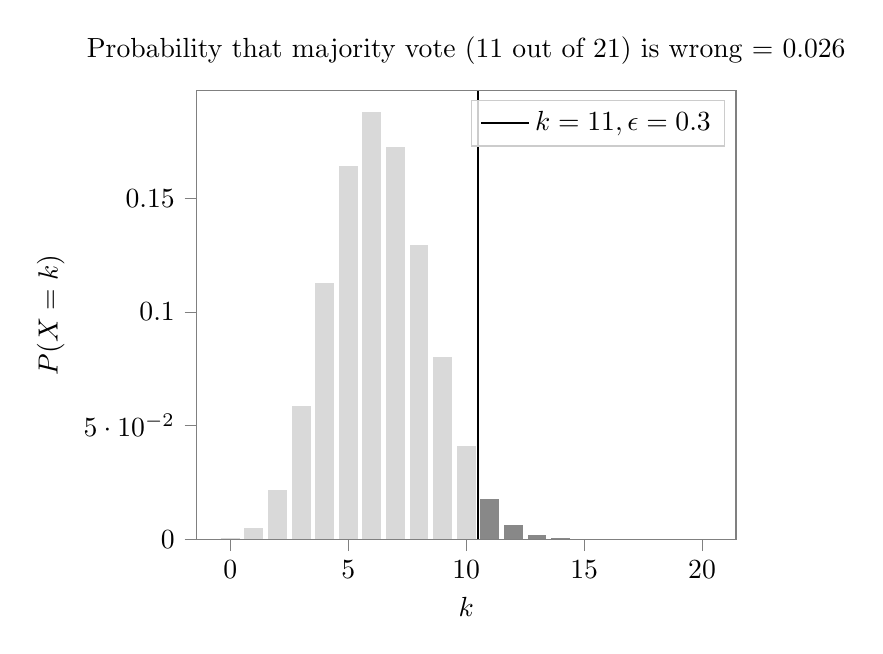
\begin{tikzpicture}

\begin{axis}[
axis line style={white!50.1960784313725!black},
legend cell align={left},
legend style={fill opacity=0.8, draw opacity=1, text opacity=1, draw=white!80!black},
tick align=outside,
tick pos=left,
title={Probability that majority vote 
 (11 out of 21) is wrong = 0.026},
x grid style={white!69.0196078431373!black},
xlabel={\(\displaystyle k\)},
xmin=-1.44, xmax=21.44,
xtick style={color=white!50.1960784313725!black},
y grid style={white!69.0196078431373!black},
ylabel={\(\displaystyle P(X=k)\)},
ymin=0, ymax=0.197196513253291,
ytick style={color=white!50.1960784313725!black}
]
\draw[draw=none,fill=white!50.1960784313725!black,fill opacity=0.3] (axis cs:-0.4,0) rectangle (axis cs:0.4,0.000558545864083285);
\draw[draw=none,fill=white!50.1960784313725!black,fill opacity=0.3] (axis cs:0.6,0) rectangle (axis cs:1.4,0.00502691277674956);
\draw[draw=none,fill=white!50.1960784313725!black,fill opacity=0.3] (axis cs:1.6,0) rectangle (axis cs:2.4,0.0215439119003552);
\draw[draw=none,fill=white!50.1960784313725!black,fill opacity=0.3] (axis cs:2.6,0) rectangle (axis cs:3.4,0.0584763323009643);
\draw[draw=none,fill=white!50.1960784313725!black,fill opacity=0.3] (axis cs:3.6,0) rectangle (axis cs:4.4,0.112775783723288);
\draw[draw=none,fill=white!50.1960784313725!black,fill opacity=0.3] (axis cs:4.6,0) rectangle (axis cs:5.4,0.164330427711076);
\draw[draw=none,fill=white!50.1960784313725!black,fill opacity=0.3] (axis cs:5.6,0) rectangle (axis cs:6.4,0.187806203098373);
\draw[draw=none,fill=white!50.1960784313725!black,fill opacity=0.3] (axis cs:6.6,0) rectangle (axis cs:7.4,0.172475084478097);
\draw[draw=none,fill=white!50.1960784313725!black,fill opacity=0.3] (axis cs:7.6,0) rectangle (axis cs:8.4,0.129356313358574);
\draw[draw=none,fill=white!50.1960784313725!black,fill opacity=0.3] (axis cs:8.6,0) rectangle (axis cs:9.4,0.0800777177934031);
\draw[draw=none,fill=white!50.1960784313725!black,fill opacity=0.3] (axis cs:9.6,0) rectangle (axis cs:10.4,0.04118282629375);
\draw[draw=none,fill=white!50.1960784313725!black,fill opacity=0.3] (axis cs:10.6,0) rectangle (axis cs:11.4,0.0176497826973214);
\draw[draw=none,fill=white!50.1960784313725!black,fill opacity=0.3] (axis cs:11.6,0) rectangle (axis cs:12.4,0.00630349382047195);
\draw[draw=none,fill=white!50.1960784313725!black,fill opacity=0.3] (axis cs:12.6,0) rectangle (axis cs:13.4,0.00187026739728288);
\draw[draw=none,fill=white!50.1960784313725!black,fill opacity=0.3] (axis cs:13.6,0) rectangle (axis cs:14.4,0.000458024668722335);
\draw[draw=none,fill=white!50.1960784313725!black,fill opacity=0.3] (axis cs:14.6,0) rectangle (axis cs:15.4,9.16049337444673e-05);
\draw[draw=none,fill=white!50.1960784313725!black,fill opacity=0.3] (axis cs:15.6,0) rectangle (axis cs:16.4,1.47222214946465e-05);
\draw[draw=none,fill=white!50.1960784313725!black,fill opacity=0.3] (axis cs:16.6,0) rectangle (axis cs:17.4,1.85574220520754e-06);
\draw[draw=none,fill=white!50.1960784313725!black,fill opacity=0.3] (axis cs:17.6,0) rectangle (axis cs:18.4,1.7673735287691e-07);
\draw[draw=none,fill=white!50.1960784313725!black,fill opacity=0.3] (axis cs:18.6,0) rectangle (axis cs:19.4,1.195967049543e-08);
\draw[draw=none,fill=white!50.1960784313725!black,fill opacity=0.3] (axis cs:19.6,0) rectangle (axis cs:20.4,5.12557306946999e-10);
\draw[draw=none,fill=white!50.1960784313725!black,fill opacity=0.9] (axis cs:10.6,0) rectangle (axis cs:11.4,0.0176497826973214);
\draw[draw=none,fill=white!50.1960784313725!black,fill opacity=0.9] (axis cs:11.6,0) rectangle (axis cs:12.4,0.00630349382047195);
\draw[draw=none,fill=white!50.1960784313725!black,fill opacity=0.9] (axis cs:12.6,0) rectangle (axis cs:13.4,0.00187026739728288);
\draw[draw=none,fill=white!50.1960784313725!black,fill opacity=0.9] (axis cs:13.6,0) rectangle (axis cs:14.4,0.000458024668722335);
\draw[draw=none,fill=white!50.1960784313725!black,fill opacity=0.9] (axis cs:14.6,0) rectangle (axis cs:15.4,9.16049337444673e-05);
\draw[draw=none,fill=white!50.1960784313725!black,fill opacity=0.9] (axis cs:15.6,0) rectangle (axis cs:16.4,1.47222214946465e-05);
\draw[draw=none,fill=white!50.1960784313725!black,fill opacity=0.9] (axis cs:16.6,0) rectangle (axis cs:17.4,1.85574220520754e-06);
\draw[draw=none,fill=white!50.1960784313725!black,fill opacity=0.9] (axis cs:17.6,0) rectangle (axis cs:18.4,1.7673735287691e-07);
\draw[draw=none,fill=white!50.1960784313725!black,fill opacity=0.9] (axis cs:18.6,0) rectangle (axis cs:19.4,1.195967049543e-08);
\draw[draw=none,fill=white!50.1960784313725!black,fill opacity=0.9] (axis cs:19.6,0) rectangle (axis cs:20.4,5.12557306946999e-10);
\addplot [thick, black]
table {%
10.5 0
10.5 0.197196513253291
};
\addlegendentry{$k=11, \epsilon=0.3$}
\end{axis}

\end{tikzpicture}

\end{frame}

\begin{frame}{Some calculations}
  \usepackage{../../shared/styles/custom}

% This file was created by tikzplotlib v0.9.0.
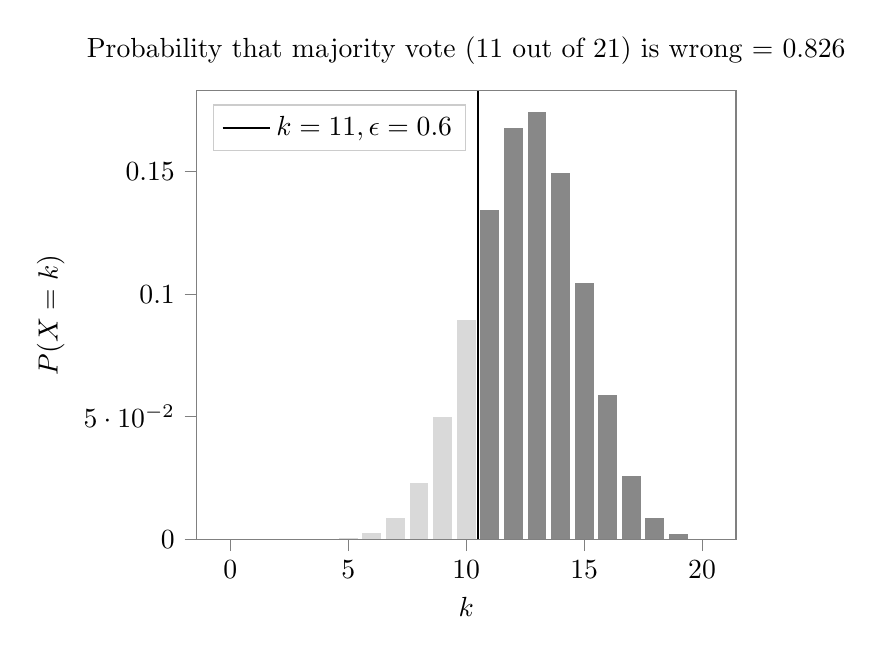
\begin{tikzpicture}

\begin{axis}[
axis line style={white!50.1960784313725!black},
legend cell align={left},
legend style={fill opacity=0.8, draw opacity=1, text opacity=1, at={(0.03,0.97)}, anchor=north west, draw=white!80!black},
tick align=outside,
tick pos=left,
title={Probability that majority vote 
 (11 out of 21) is wrong = 0.826},
x grid style={white!69.0196078431373!black},
xlabel={\(\displaystyle k\)},
xmin=-1.44, xmax=21.44,
xtick style={color=white!50.1960784313725!black},
y grid style={white!69.0196078431373!black},
ylabel={\(\displaystyle P(X=k)\)},
ymin=0, ymax=0.182885197845734,
ytick style={color=white!50.1960784313725!black}
]
\draw[draw=none,fill=white!50.1960784313725!black,fill opacity=0.3] (axis cs:-0.4,0) rectangle (axis cs:0.4,4.39804651110401e-09);
\draw[draw=none,fill=white!50.1960784313725!black,fill opacity=0.3] (axis cs:0.6,0) rectangle (axis cs:1.4,1.38538465099776e-07);
\draw[draw=none,fill=white!50.1960784313725!black,fill opacity=0.3] (axis cs:1.6,0) rectangle (axis cs:2.4,2.07807697649663e-06);
\draw[draw=none,fill=white!50.1960784313725!black,fill opacity=0.3] (axis cs:2.6,0) rectangle (axis cs:3.4,1.97417312767181e-05);
\draw[draw=none,fill=white!50.1960784313725!black,fill opacity=0.3] (axis cs:3.6,0) rectangle (axis cs:4.4,0.000133256686117847);
\draw[draw=none,fill=white!50.1960784313725!black,fill opacity=0.3] (axis cs:4.6,0) rectangle (axis cs:5.4,0.000679609099201017);
\draw[draw=none,fill=white!50.1960784313725!black,fill opacity=0.3] (axis cs:5.6,0) rectangle (axis cs:6.4,0.00271843639680407);
\draw[draw=none,fill=white!50.1960784313725!black,fill opacity=0.3] (axis cs:6.6,0) rectangle (axis cs:7.4,0.00873783127544164);
\draw[draw=none,fill=white!50.1960784313725!black,fill opacity=0.3] (axis cs:7.6,0) rectangle (axis cs:8.4,0.0229368070980344);
\draw[draw=none,fill=white!50.1960784313725!black,fill opacity=0.3] (axis cs:8.6,0) rectangle (axis cs:9.4,0.0496964153790748);
\draw[draw=none,fill=white!50.1960784313725!black,fill opacity=0.3] (axis cs:9.6,0) rectangle (axis cs:10.4,0.0894535476823343);
\draw[draw=none,fill=white!50.1960784313725!black,fill opacity=0.3] (axis cs:10.6,0) rectangle (axis cs:11.4,0.134180321523501);
\draw[draw=none,fill=white!50.1960784313725!black,fill opacity=0.3] (axis cs:11.6,0) rectangle (axis cs:12.4,0.167725401904377);
\draw[draw=none,fill=white!50.1960784313725!black,fill opacity=0.3] (axis cs:12.6,0) rectangle (axis cs:13.4,0.174176378900699);
\draw[draw=none,fill=white!50.1960784313725!black,fill opacity=0.3] (axis cs:13.6,0) rectangle (axis cs:14.4,0.149294039057741);
\draw[draw=none,fill=white!50.1960784313725!black,fill opacity=0.3] (axis cs:14.6,0) rectangle (axis cs:15.4,0.104505827340419);
\draw[draw=none,fill=white!50.1960784313725!black,fill opacity=0.3] (axis cs:15.6,0) rectangle (axis cs:16.4,0.0587845278789856);
\draw[draw=none,fill=white!50.1960784313725!black,fill opacity=0.3] (axis cs:16.6,0) rectangle (axis cs:17.4,0.0259343505348466);
\draw[draw=none,fill=white!50.1960784313725!black,fill opacity=0.3] (axis cs:17.6,0) rectangle (axis cs:18.4,0.00864478351161558);
\draw[draw=none,fill=white!50.1960784313725!black,fill opacity=0.3] (axis cs:18.6,0) rectangle (axis cs:19.4,0.00204744872643526);
\draw[draw=none,fill=white!50.1960784313725!black,fill opacity=0.3] (axis cs:19.6,0) rectangle (axis cs:20.4,0.00030711730896529);
\draw[draw=none,fill=white!50.1960784313725!black,fill opacity=0.9] (axis cs:10.6,0) rectangle (axis cs:11.4,0.134180321523501);
\draw[draw=none,fill=white!50.1960784313725!black,fill opacity=0.9] (axis cs:11.6,0) rectangle (axis cs:12.4,0.167725401904377);
\draw[draw=none,fill=white!50.1960784313725!black,fill opacity=0.9] (axis cs:12.6,0) rectangle (axis cs:13.4,0.174176378900699);
\draw[draw=none,fill=white!50.1960784313725!black,fill opacity=0.9] (axis cs:13.6,0) rectangle (axis cs:14.4,0.149294039057741);
\draw[draw=none,fill=white!50.1960784313725!black,fill opacity=0.9] (axis cs:14.6,0) rectangle (axis cs:15.4,0.104505827340419);
\draw[draw=none,fill=white!50.1960784313725!black,fill opacity=0.9] (axis cs:15.6,0) rectangle (axis cs:16.4,0.0587845278789856);
\draw[draw=none,fill=white!50.1960784313725!black,fill opacity=0.9] (axis cs:16.6,0) rectangle (axis cs:17.4,0.0259343505348466);
\draw[draw=none,fill=white!50.1960784313725!black,fill opacity=0.9] (axis cs:17.6,0) rectangle (axis cs:18.4,0.00864478351161558);
\draw[draw=none,fill=white!50.1960784313725!black,fill opacity=0.9] (axis cs:18.6,0) rectangle (axis cs:19.4,0.00204744872643526);
\draw[draw=none,fill=white!50.1960784313725!black,fill opacity=0.9] (axis cs:19.6,0) rectangle (axis cs:20.4,0.00030711730896529);
\addplot [thick, black]
table {%
10.5 -3.46944695195361e-18
10.5 0.182885197845734
};
\addlegendentry{$k=11, \epsilon=0.6$}
\end{axis}

\end{tikzpicture}

\end{frame}
\begin{frame}{Ensemble Methods}
  \only<1->{
    Where does ensemble learning not work well?
  }
  \only<2->{
    \begin{itemize}
      \item The base model is bad.
      \item All models give similar prediction or the models are highly correlated.
    \end{itemize}
  }
\end{frame}

\begin{frame}{Bagging}
  \only<1->{
    Also known as $Bootstrap$ $Aggregation$.\\
  }
  \only<2->{
    $Key$ $idea$ : Reduce Variance\\
    \vspace{1cm}
  }
  \only<3->{
    How to learn different classifiers while feeding in the same data?\\
    \vspace{0.5cm}
  }
  \only<4->{
    Think about cross-validation!\\
    \vspace{0.5cm}
  }
  \only<5->{
    We will create multiple datasets from our single dataset using ``$sampling$ $with$ $replacement$''.
  }
\end{frame}

\begin{frame}{Bagging}
  \only<1->{
    Consider our dataset has $n$ samples, $D_1, D_2, D_3, \dots, D_n$.\\
    For each model in the ensemble, we create a new dataset of size $n$ by sampling uniformly with replacement.\\
    \vspace{1cm}
  }
  \only<2->{
    Round 1 : $D_1, D_3, D_6, D_1, \dots, D_n$\\
    Round 2 : $D_2, D_4, D_1, D_{80}, \dots, D_3$\\
    \vdots
  }
  \only<3->{
    Repetition of samples is possible.\\
  }
  \only<4->{
    We can train the same classifier/models on each of these different ``Bagging Rounds''.
  }
\end{frame}

\begin{frame}{Bagging : Classification Example}     % remiaining - start
  Consider the dataset below. Points (3,3) and (5,8) are anomalies.\\
  \vspace{0.5cm}
  \centering
  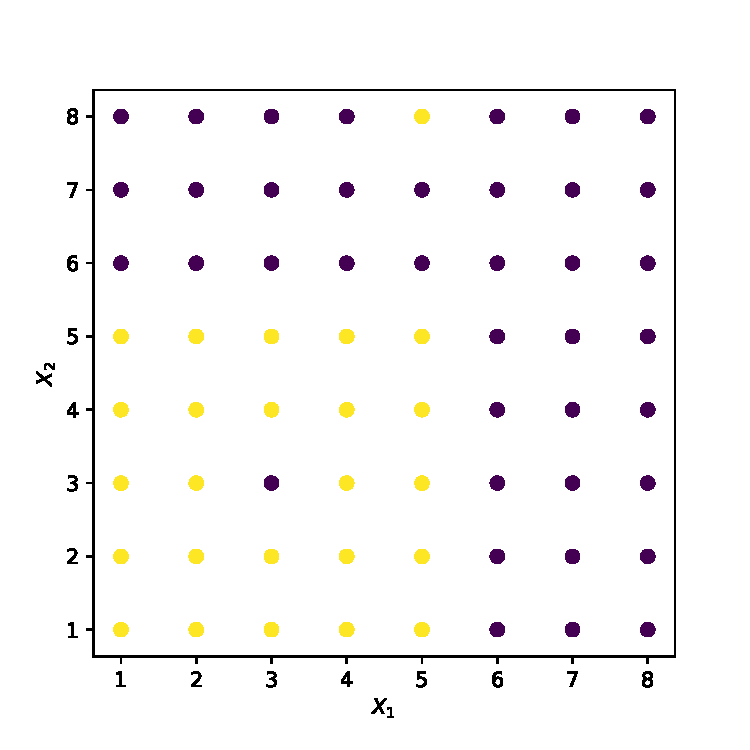
\includegraphics[width = 0.6\textwidth]{../assets/ensemble/figures/dataset}
\end{frame}


\begin{frame}{Bagging : Classification Example}
  Decision Boundary for decision tree with depth 6.\\
  \vspace{0.5cm}
  \centering
  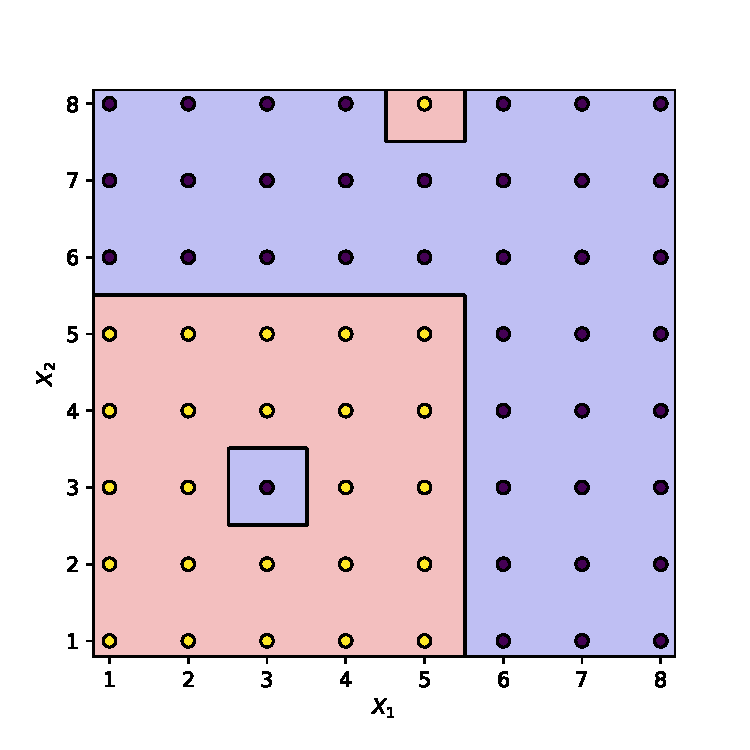
\includegraphics[width = 0.6\textwidth]{../assets/ensemble/figures/strong-tree}
\end{frame}

\begin{frame}{Bagging : Classification Example}
  Lets use bagging with ensemble of 5 trees.\\
  \vspace{0.5cm}
  \begin{columns}
    \pause  \begin{column}{0.3\textwidth}
      \centering
      Round - 1\\

      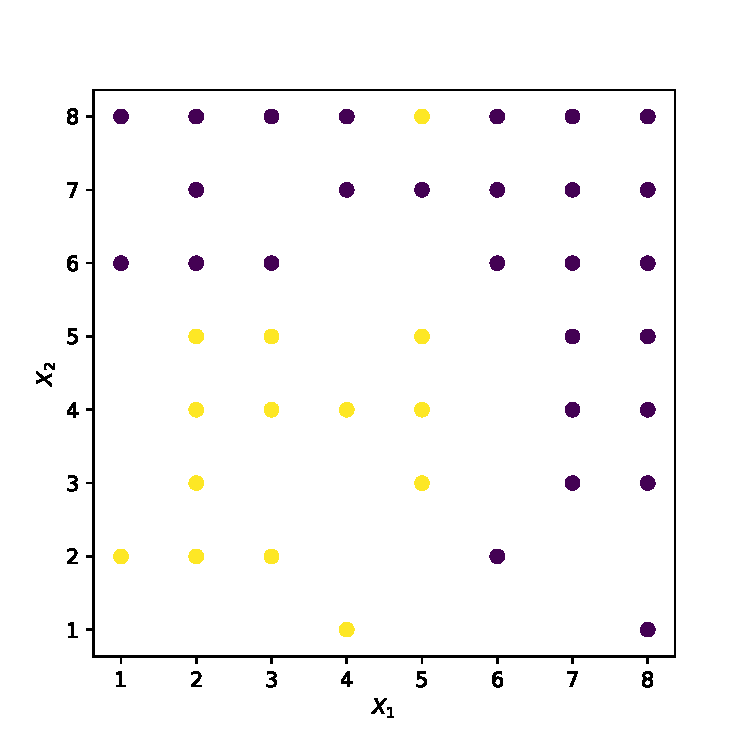
\includegraphics[width = 0.9\textwidth]{../assets/ensemble/figures/dataset-rnd-0}

    \end{column}
    \pause  \begin{column}{0.3\textwidth}
      \centering
      Round - 2\\

      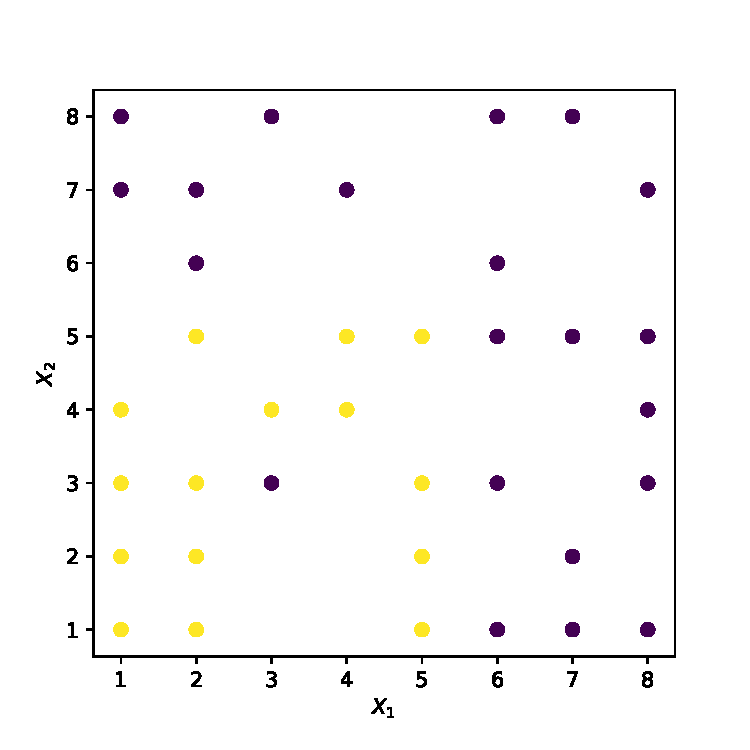
\includegraphics[width = 0.9\textwidth]{../assets/ensemble/figures/dataset-rnd-1}

    \end{column}
    \pause  \begin{column}{0.3\textwidth}
      \centering
      Round - 3\\

      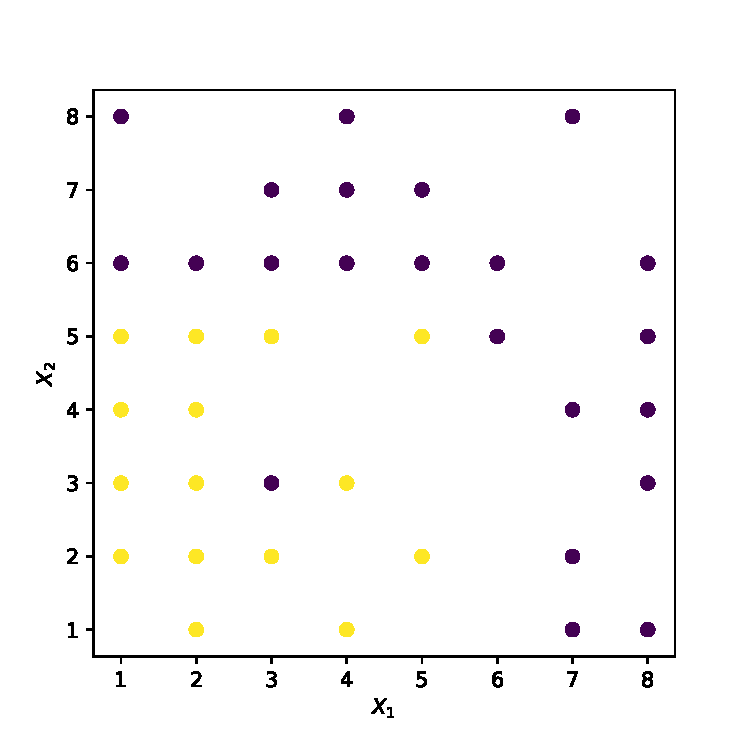
\includegraphics[width = 0.9\textwidth]{../assets/ensemble/figures/dataset-rnd-2}

    \end{column}

  \end{columns}
  \vspace{0.5cm}
  \begin{columns}
    \pause  \begin{column}{0.3\textwidth}
      \centering
      Round - 4\\

      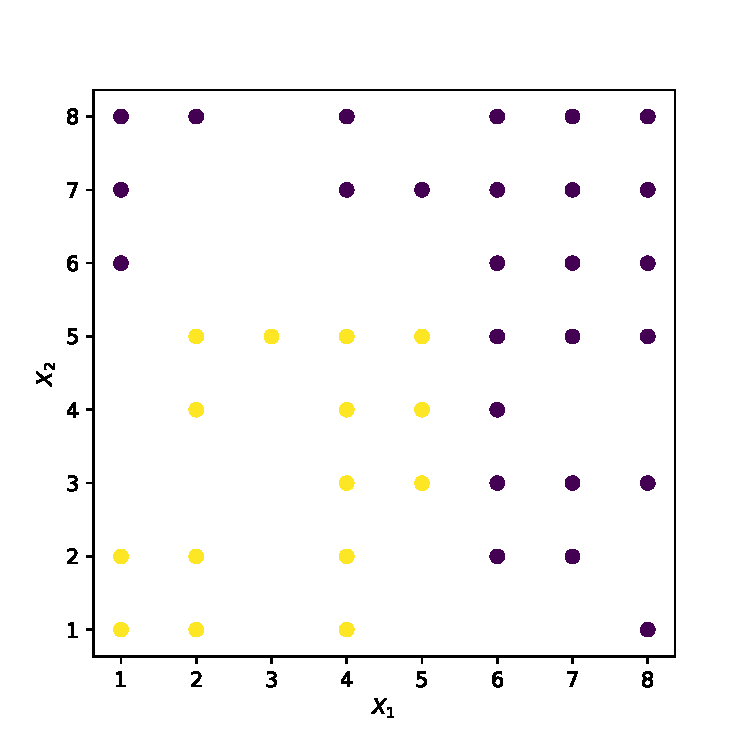
\includegraphics[width = 0.9\textwidth]{../assets/ensemble/figures/dataset-rnd-3}

    \end{column}
    \pause  \begin{column}{0.3\textwidth}
      \centering
      Round - 5\\

      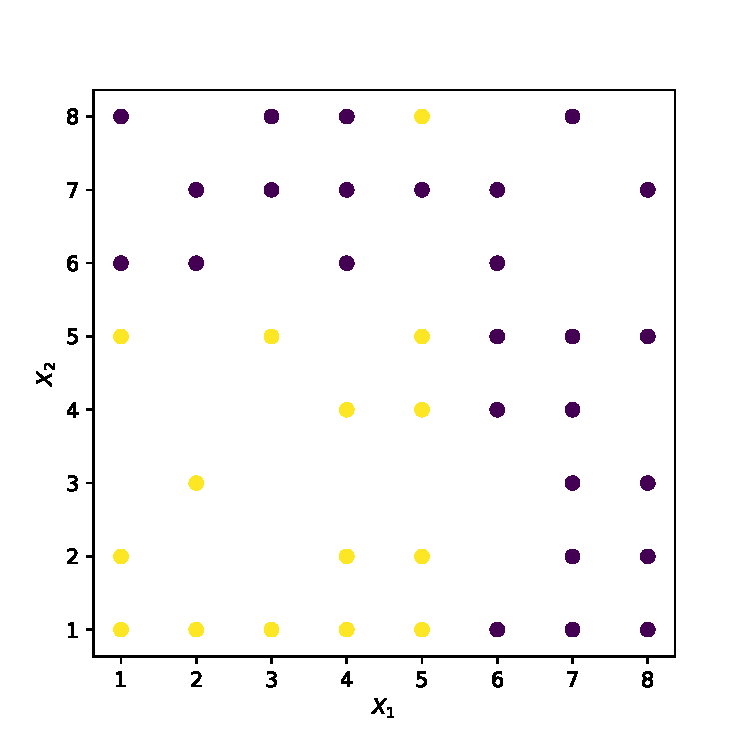
\includegraphics[width = 0.9\textwidth]{../assets/ensemble/figures/dataset-rnd-4}

    \end{column}

  \end{columns}
\end{frame}


\begin{frame}{Bagging : Classification Example}
  \vspace{0.3cm}
  \begin{columns}
    \pause  \begin{column}{0.3\textwidth}
      \centering
      Round - 1\\

      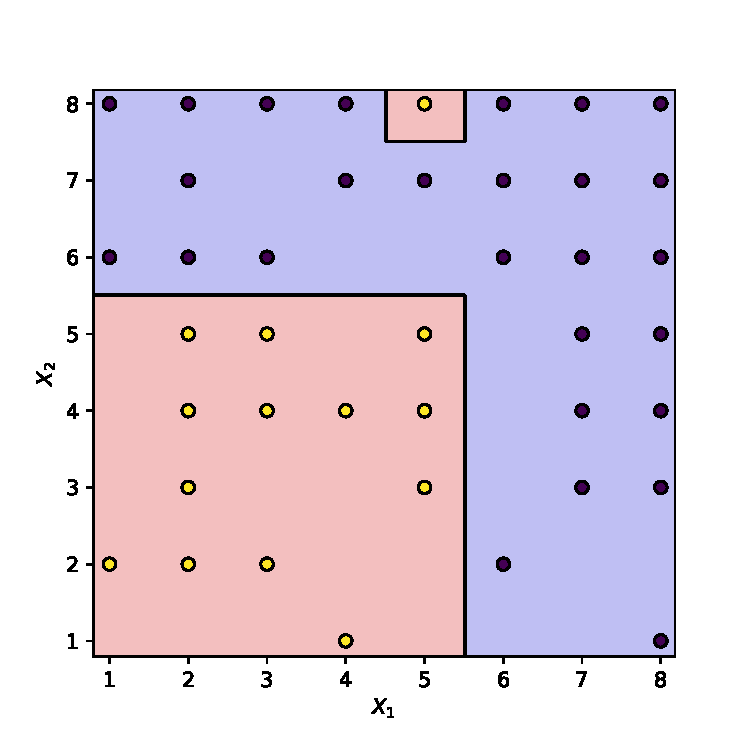
\includegraphics[width = 0.9\textwidth]{../assets/ensemble/figures/decision-boundary-0}
      Tree Depth = 4

    \end{column}
    \pause  \begin{column}{0.3\textwidth}
      \centering
      Round - 2\\

      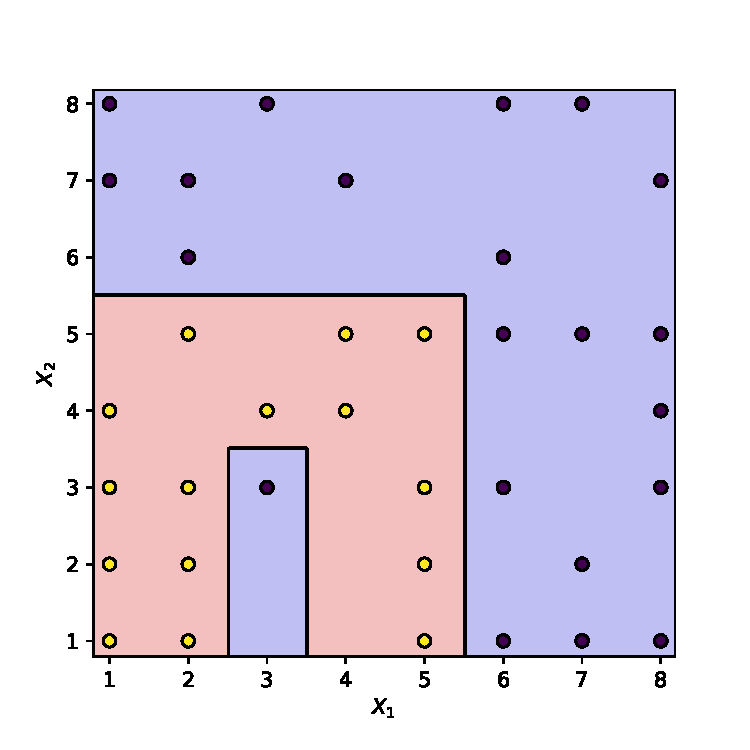
\includegraphics[width = 0.9\textwidth]{../assets/ensemble/figures/decision-boundary-1}
      Tree Depth = 5

    \end{column}
    \pause  \begin{column}{0.3\textwidth}
      \centering
      Round - 3\\

      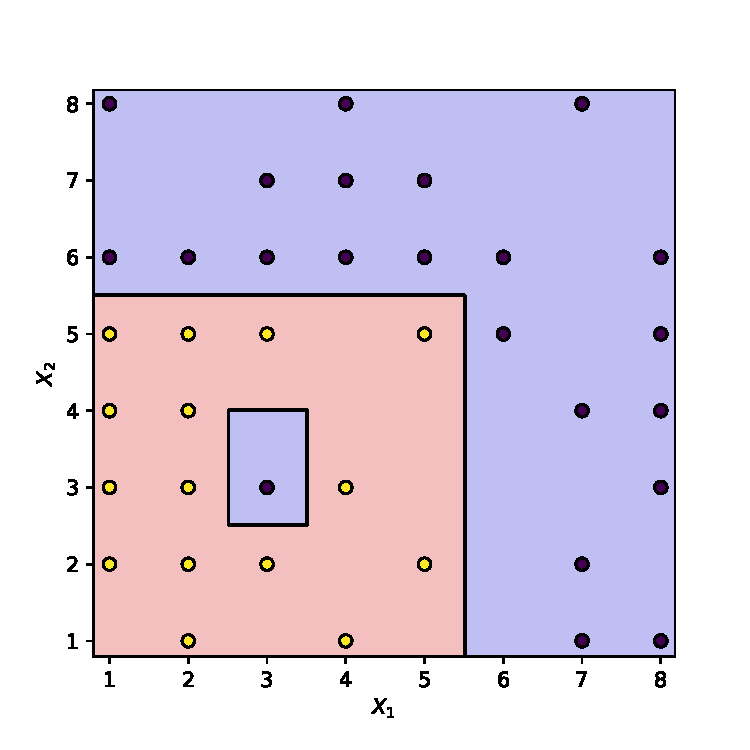
\includegraphics[width = 0.9\textwidth]{../assets/ensemble/figures/decision-boundary-2}
      Tree Depth = 5

    \end{column}

  \end{columns}
  \vspace{0.5cm}
  \pause  \begin{columns}
    \begin{column}{0.3\textwidth}
      \centering
      Round - 4\\

      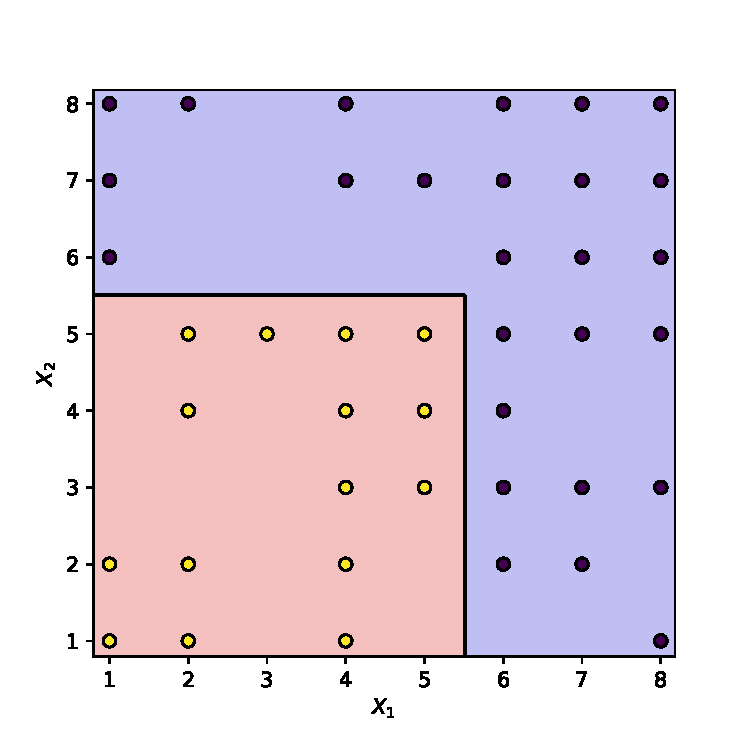
\includegraphics[width = 0.9\textwidth]{../assets/ensemble/figures/decision-boundary-3}
      Tree Depth = 2

    \end{column}
    \pause  \begin{column}{0.3\textwidth}
      \centering
      Round - 5\\

      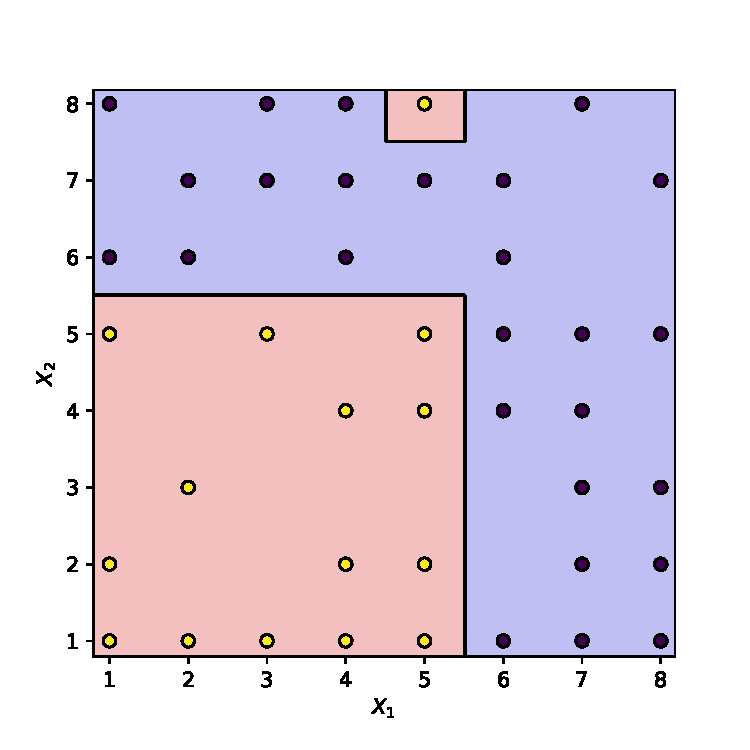
\includegraphics[width = 0.9\textwidth]{../assets/ensemble/figures/decision-boundary-4}
      Tree Depth = 4

    \end{column}

  \end{columns}
\end{frame}

\begin{frame}{Bagging : Classification Example}
  Using majority voting to combine all predictions, we get the decision boundary below.\\
  \vspace{0.5cm}
  \centering
  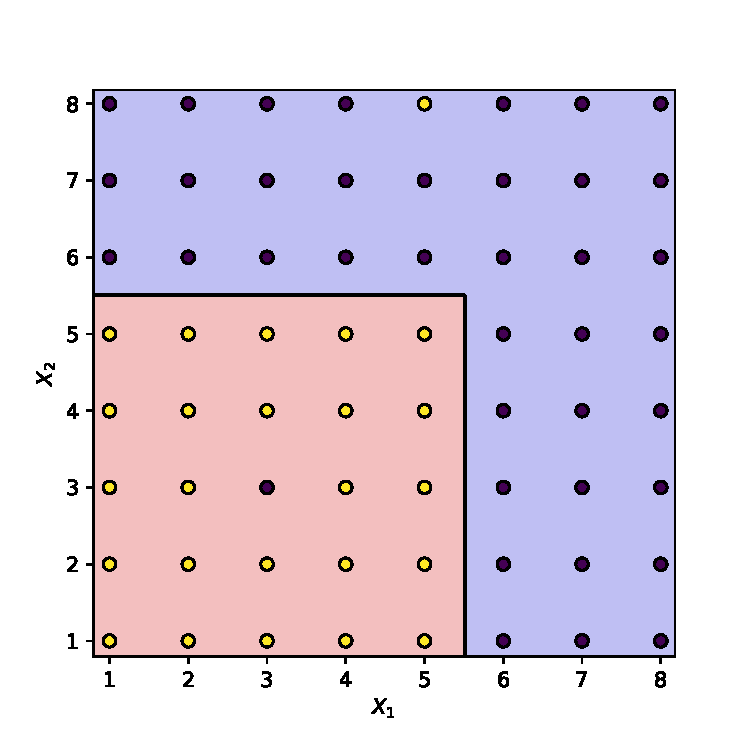
\includegraphics[width = 0.6\textwidth]{../assets/ensemble/figures/decision-boundary-ensemble}
\end{frame}

\begin{frame}{Bagging}
  \textbf{Summary}
  \begin{itemize}
    \item We take ``strong'' learners and combine them to reduce variance.
    \item All learners are independent of each other.
  \end{itemize}
\end{frame}

\begin{frame}{Boosting}
  \begin{itemize}
    \item We take ``weak'' learners and combine them to reduce bias.
          \pause \item All learners are incrementally built.
          \pause \item Incremental building: Incrementally try to classify ``harder'' samples correctly.
  \end{itemize}
\end{frame}

\begin{frame}{Boosting : AdaBoost }
  Consider we have a dataset of $N$ samples.\\
  Sample $i$ has weight $w_i$. There are $M$ classifers in ensemble.\\
  \vspace{0.5cm}
  \centering
  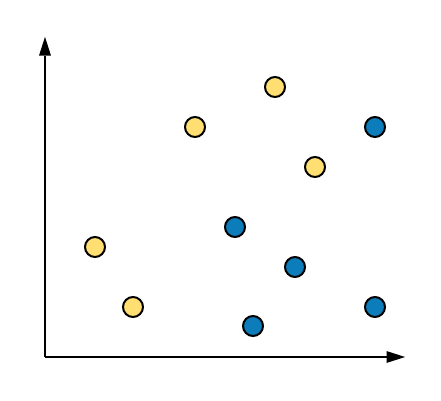
\includegraphics[width = 0.6\textwidth]{../assets/ensemble/diagrams/ada_data}
\end{frame}

\begin{frame}{Boosting : AdaBoost }
  Consider we have a dataset of $N$ samples.\\
  Sample $i$ has weight $w_i$. There are $M$ classifers in ensemble.\\
  \begin{enumerate}
    \item Initialize weights of data samples, $w_i = \dfrac{1}{N}$
  \end{enumerate}
  \vspace{0.5cm}
  \centering
  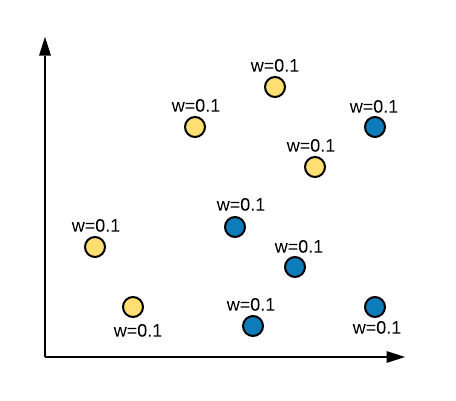
\includegraphics[width = 0.6\textwidth]{../assets/ensemble/diagrams/ada_data_init_weights}
\end{frame}

\begin{frame}{Boosting : AdaBoost }
  Consider we have a dataset of $N$ samples.\\
  Sample $i$ has weight $w_i$. There are $M$ classifers in ensemble.\\
  \begin{enumerate}
    \item Initialize weights of data samples, $w_i = \dfrac{1}{N}$
    \item For $m = 1\dots M$
          \begin{enumerate}
            \item Learn classifier using current weights $w_i's$
          \end{enumerate}
  \end{enumerate}
  \centering
  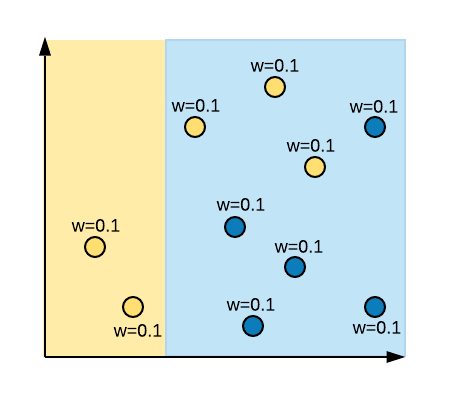
\includegraphics[width = 0.6\textwidth]{../assets/ensemble/diagrams/ada_iter1}
\end{frame}

\begin{frame}{Boosting : AdaBoost }
  Consider we have a dataset of $N$ samples.\\
  Sample $i$ has weight $w_i$. There are $M$ classifers in ensemble.\\
  \begin{enumerate}
    \item Initialize weights of data samples, $w_i = \dfrac{1}{N}$
    \item For $m = 1\dots M$
          \begin{enumerate}
            \item Learn classifier using current weights $w_i's$
          \end{enumerate}
  \end{enumerate}
  \centering
  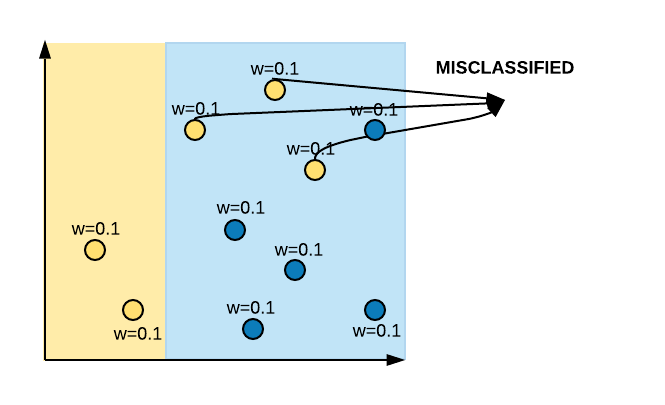
\includegraphics[width = 0.85\textwidth]{../assets/ensemble/diagrams/ada_iter1_misclassify}
\end{frame}

\begin{frame}{Boosting : AdaBoost }
  Consider we have a dataset of $N$ samples.\\
  Sample $i$ has weight $w_i$. There are $M$ classifers in ensemble.\\
  \begin{enumerate}
    \item Initialize weights of data samples, $w_i = \dfrac{1}{N}$
    \item For $m = 1\dots M$
          \begin{enumerate}
            \item Learn classifier using current weights $w_i's$
            \item Compute the weighted error, $err_m = \dfrac{\sum\limits_iw_i(incorrect)}{\sum\limits_iw_i}$
          \end{enumerate}
  \end{enumerate}
  \begin{columns}
    \begin{column}{0.5\textwidth}
      \centering
      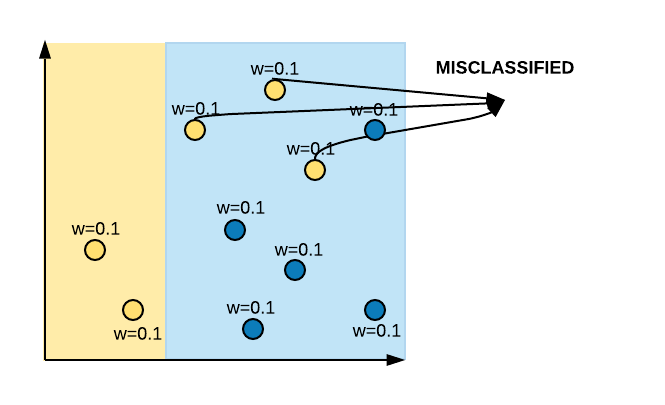
\includegraphics[width = 1.1\textwidth]{../assets/ensemble/diagrams/ada_iter1_misclassify}
    \end{column}
    \begin{column}{0.5\textwidth}
      $err_1 = \dfrac{0.3}{1}$
    \end{column}
  \end{columns}
\end{frame}


\begin{frame}{Boosting : AdaBoost }
  Consider we have a dataset of $N$ samples.\\
  Sample $i$ has weight $w_i$. There are $M$ classifers in ensemble.\\
  \begin{enumerate}
    \item Initialize weights of data samples, $w_i = \dfrac{1}{N}$
    \item For $m = 1\dots M$
          \begin{enumerate}
            \item Learn classifier using current weights $w_i's$
            \item Compute the weighted error, $err_m = \dfrac{\sum\limits_iw_i(incorrect)}{\sum\limits_iw_i}$
            \item Compute $\alpha_m = \dfrac{1}{2}log_e\left(\dfrac{1 - err_m}{err_m}\right)$
          \end{enumerate}
  \end{enumerate}
  \begin{columns}
    \begin{column}{0.5\textwidth}
      \centering
      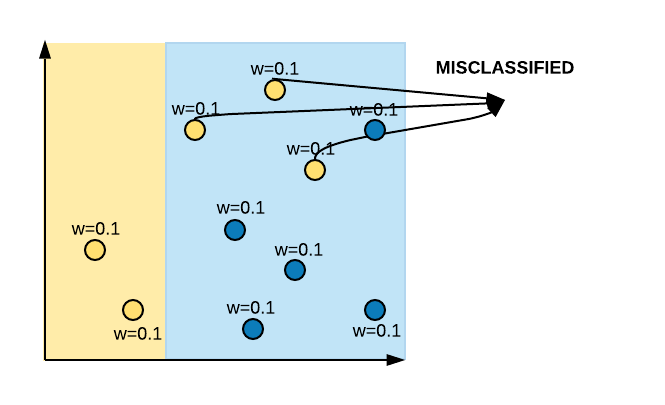
\includegraphics[width = \textwidth]{../assets/ensemble/diagrams/ada_iter1_misclassify}
    \end{column}
    \begin{column}{0.5\textwidth}
      $err_1 = \dfrac{0.3}{1}$\\
      $\alpha_1 = \dfrac{1}{2}log\left(\dfrac{1-0.3}{0.3}\right) = 0.42$
    \end{column}
  \end{columns}
\end{frame}

\begin{frame}{Boosting : AdaBoost }
  Consider we have a dataset of $N$ samples.\\
  Sample $i$ has weight $w_i$. There are $M$ classifers in ensemble.\\
  \begin{enumerate}
    \item Initialize weights of data samples, $w_i = \dfrac{1}{N}$
    \item For $m = 1\dots M$
          \begin{enumerate}
            \item Learn classifier using current weights $w_i's$
            \item Compute the weighted error, $err_m = \dfrac{\sum\limits_iw_i(incorrect)}{\sum\limits_iw_i}$
            \item Compute $\alpha_m = \dfrac{1}{2}log_e\left(\dfrac{1 - err_m}{err_m}\right)$
            \item For samples which were predicted correctly, $w_i = w_ie^{-\alpha_m}$
            \item For samples which were predicted incorrectly, $w_i = w_ie^{\alpha_m}$
          \end{enumerate}
  \end{enumerate}
\end{frame}

\begin{frame}{Boosting : AdaBoost }
  \vspace{0.5cm}
  \centering
  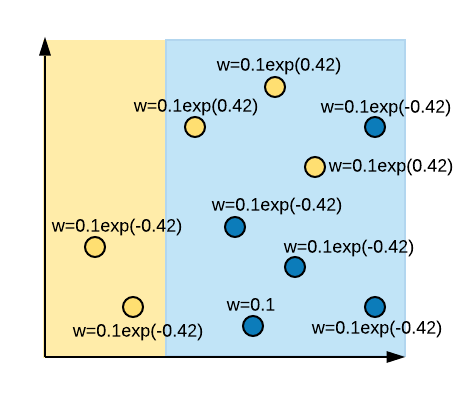
\includegraphics[width = 0.8\textwidth]{../assets/ensemble/diagrams/ada_iter1_new_weights_exp}
\end{frame}

\begin{frame}{Boosting : AdaBoost }
  \vspace{0.5cm}
  \centering
  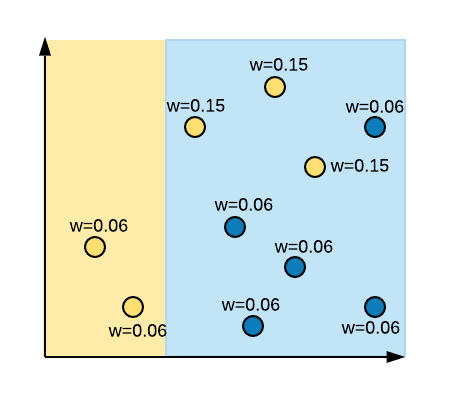
\includegraphics[width = 0.8\textwidth]{../assets/ensemble/diagrams/ada_iter1_new_weights}
\end{frame}

\begin{frame}{Boosting : AdaBoost }
  Consider we have a dataset of $N$ samples.\\
  Sample $i$ has weight $w_i$. There are $M$ classifers in ensemble.\\
  \begin{enumerate}
    \item Initialize weights of data samples, $w_i = \dfrac{1}{N}$
    \item For $m = 1\dots M$
          \begin{enumerate}
            \item Learn classifier using current weights $w_i's$
            \item Compute the weighted error, $err_m = \dfrac{\sum\limits_iw_i(incorrect)}{\sum\limits_iw_i}$
            \item Compute $\alpha_m = \dfrac{1}{2}log_e\left(\dfrac{1 - err_m}{err_m}\right)$
            \item For samples which were predicted correctly, $w_i = w_ie^{-\alpha_m}$
            \item For samples which were predicted incorrectly, $w_i = w_ie^{\alpha_m}$
            \item Normalize $w_i's$ to sum up to 1.
          \end{enumerate}
  \end{enumerate}
\end{frame}

\begin{frame}{Boosting : AdaBoost }
  \vspace{0.5cm}
  \centering
  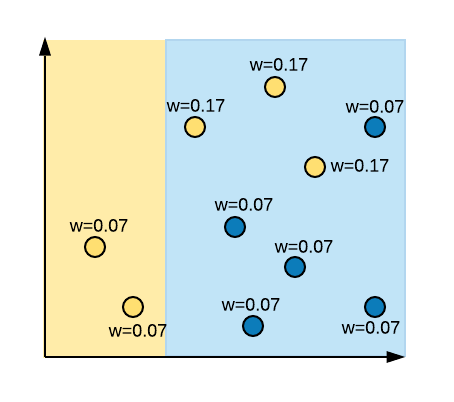
\includegraphics[width = 0.8\textwidth]{../assets/ensemble/diagrams/ada_iter1_new_weights_normalized}
\end{frame}


\begin{frame}{Boosting : AdaBoost }
  Consider we have a dataset of $N$ samples.\\
  Sample $i$ has weight $w_i$. There are $M$ classifers in ensemble.\\
  \begin{enumerate}
    \item Initialize weights of data samples, $w_i = \dfrac{1}{N}$
    \item For $m = 1\dots M$
          \begin{enumerate}
            \item Learn classifier using current weights $w_i's$
            \item Compute the weighted error, $err_m = \dfrac{\sum\limits_iw_i(incorrect)}{\sum\limits_iw_i}$
            \item Compute $\alpha_m = \dfrac{1}{2}log_e\left(\dfrac{1 - err_m}{err_m}\right)$
          \end{enumerate}
  \end{enumerate}
  \begin{columns}
    \begin{column}{0.5\textwidth}
      \centering
      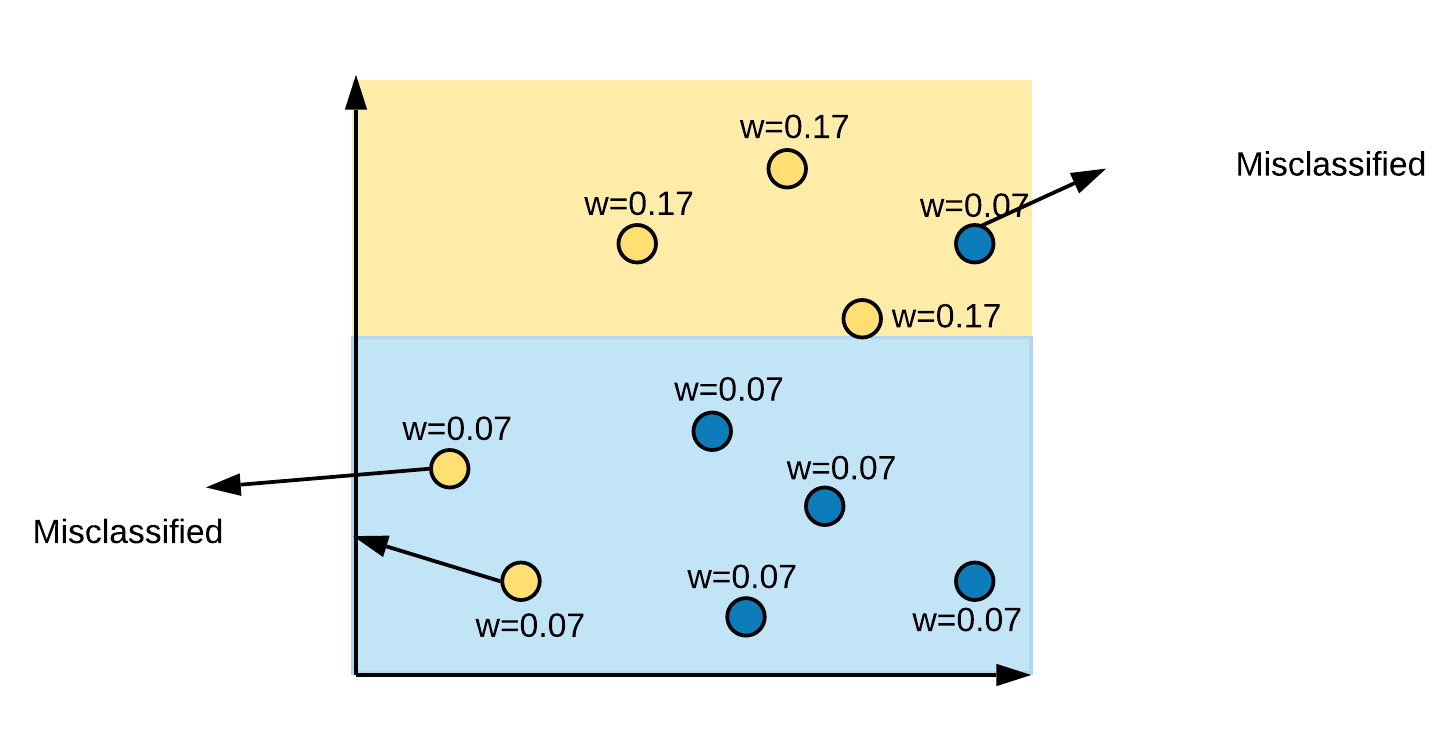
\includegraphics[width = \textwidth]{../assets/ensemble/diagrams/ada_iter2_misclassify}
    \end{column}
    \begin{column}{0.5\textwidth}
      $err_2 = \dfrac{0.21}{1}$\\
      $\alpha_2 = \dfrac{1}{2}log\left(\dfrac{1-0.21}{0.21}\right) = 0.66$
    \end{column}
  \end{columns}
\end{frame}

\begin{frame}{Boosting : AdaBoost }
  Consider we have a dataset of $N$ samples.\\
  Sample $i$ has weight $w_i$. There are $M$ classifers in ensemble.\\
  \begin{enumerate}
    \item Initialize weights of data samples, $w_i = \dfrac{1}{N}$
    \item For $m = 1\dots M$
          \begin{enumerate}
            \item Learn classifier using current weights $w_i's$
            \item Compute the weighted error, $err_m = \dfrac{\sum\limits_iw_i(incorrect)}{\sum\limits_iw_i}$
            \item Compute $\alpha_m = \dfrac{1}{2}log_e\left(\dfrac{1 - err_m}{err_m}\right)$
            \item For samples which were predicted correctly, $w_i = w_ie^{-\alpha_m}$
            \item For samples which were predicted incorrectly, $w_i = w_ie^{\alpha_m}$
          \end{enumerate}
  \end{enumerate}
\end{frame}

\begin{frame}{Boosting : AdaBoost }
  \vspace{0.5cm}
  \centering
  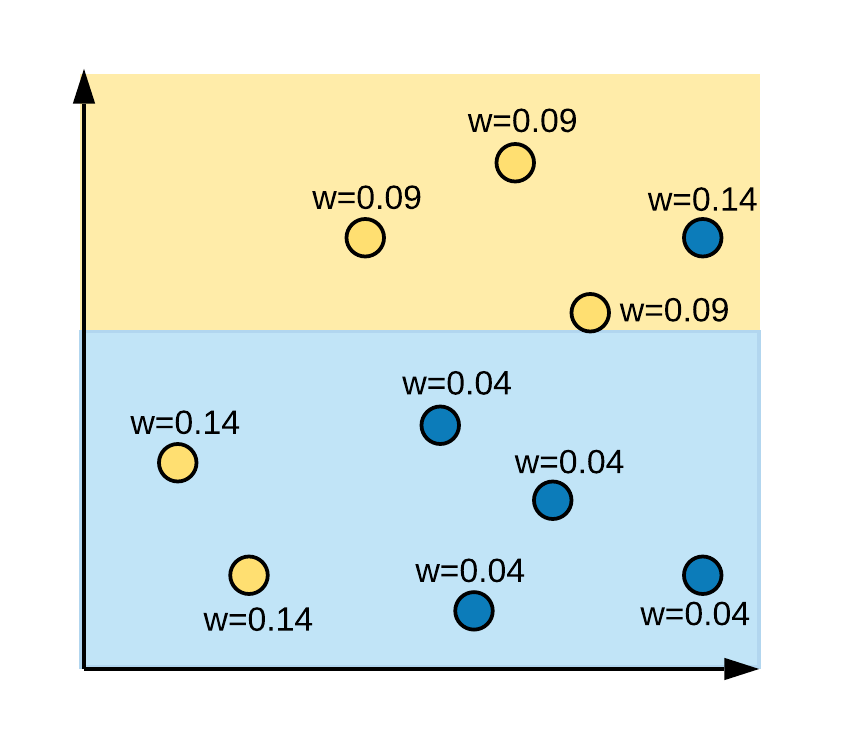
\includegraphics[width = 0.8\textwidth]{../assets/ensemble/diagrams/ada_iter2_new_weights}
\end{frame}

\begin{frame}{Boosting : AdaBoost }
  Consider we have a dataset of $N$ samples.\\
  Sample $i$ has weight $w_i$. There are $M$ classifers in ensemble.\\
  \begin{enumerate}
    \item Initialize weights of data samples, $w_i = \dfrac{1}{N}$
    \item For $m = 1\dots M$
          \begin{enumerate}
            \item Learn classifier using current weights $w_i's$
            \item Compute the weighted error, $err_m = \dfrac{\sum\limits_iw_i(incorrect)}{\sum\limits_iw_i}$
            \item Compute $\alpha_m = \dfrac{1}{2}log_e\left(\dfrac{1 - err_m}{err_m}\right)$
            \item For samples which were predicted correctly, $w_i = w_ie^{-\alpha_m}$
            \item For samples which were predicted incorrectly, $w_i = w_ie^{\alpha_m}$
            \item Normalize $w_i's$ to sum up to 1.
          \end{enumerate}
  \end{enumerate}
\end{frame}

\begin{frame}{Boosting : AdaBoost }
  \vspace{0.5cm}
  \centering
  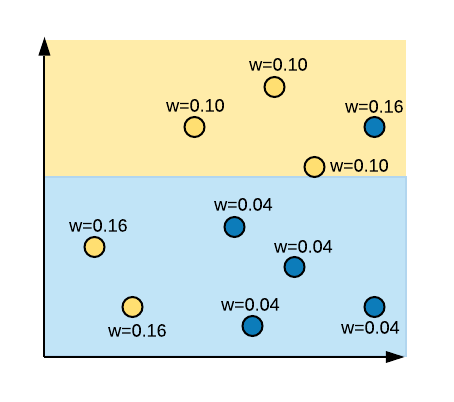
\includegraphics[width = 0.8\textwidth]{../assets/ensemble/diagrams/ada_iter2_new_weights_normalized}
\end{frame}


\begin{frame}{Boosting : AdaBoost }
  Consider we have a dataset of $N$ samples.\\
  Sample $i$ has weight $w_i$. There are $M$ classifers in ensemble.\\
  \begin{enumerate}
    \item Initialize weights of data samples, $w_i = \dfrac{1}{N}$
    \item For $m = 1\dots M$
          \begin{enumerate}
            \item Learn classifier using current weights $w_i's$
            \item Compute the weighted error, $err_m = \dfrac{\sum\limits_iw_i(incorrect)}{\sum\limits_iw_i}$
            \item Compute $\alpha_m = \dfrac{1}{2}log_e\left(\dfrac{1 - err_m}{err_m}\right)$
          \end{enumerate}
  \end{enumerate}
  \begin{columns}
    \begin{column}{0.5\textwidth}
      \centering
      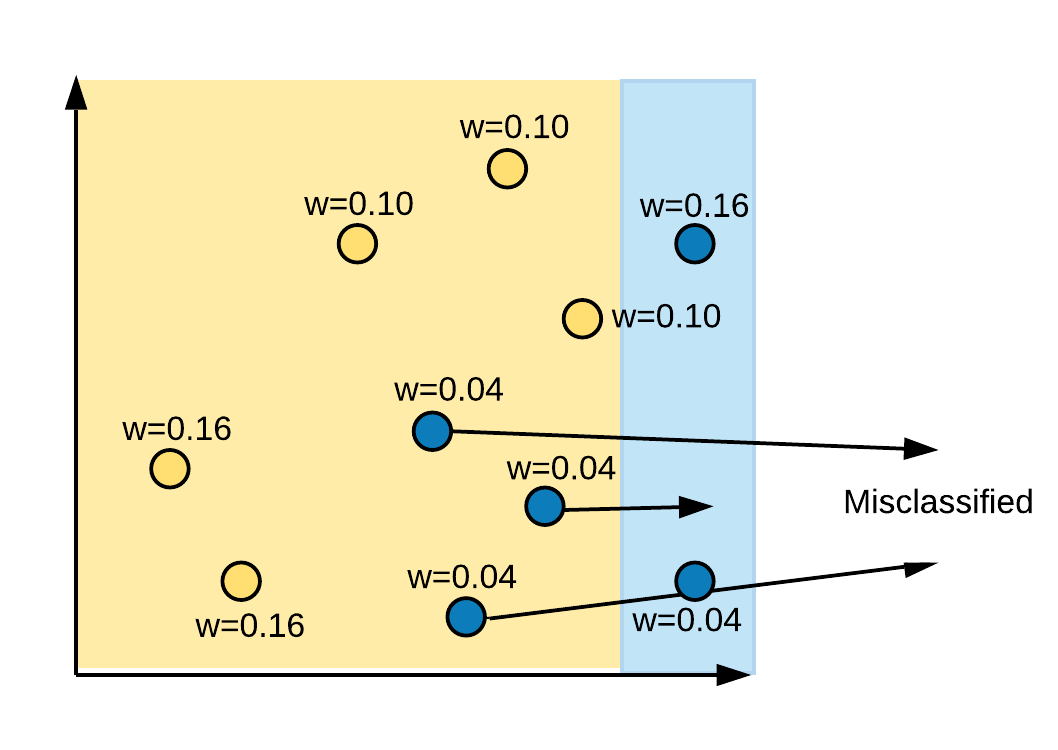
\includegraphics[width = \textwidth]{../assets/ensemble/diagrams/ada_iter3_misclassify}
    \end{column}
    \begin{column}{0.5\textwidth}
      $err_3 = \dfrac{0.12}{1}$\\
      $\alpha_3 = \dfrac{1}{2}log\left(\dfrac{1-0.12}{0.12}\right) = 0.99$
    \end{column}
  \end{columns}
\end{frame}

\begin{frame}{Boosting: Adaboost}
  Intuitively, after each iteration, importance of wrongly classified samples is increased by increasing their weights and importance of correctly classified     samples is decreased by decreasing their weights.
\end{frame}

\begin{frame}{Boosting: Adaboost}
  \textbf{Testing}\\
  \begin{itemize}
	\item For each sample $x$, compute the prediction of each classifier $h_m(x)$.
	\item Final prediction is the sign of the sum of weighted predictions, given as:
	\item SIGN($\alpha_1 h_1(x)$ +  $\alpha_2 h_2(x)$ + $\dots$ +  $\alpha_M h_M(x)$)
  \end{itemize}

\end{frame}

\begin{frame}{Boosting: Adaboost}
  \textbf{Example}
	\begin{columns}
		\pause 			\begin{column}{0.33\textwidth}
				\centering
				\begin{figure}
					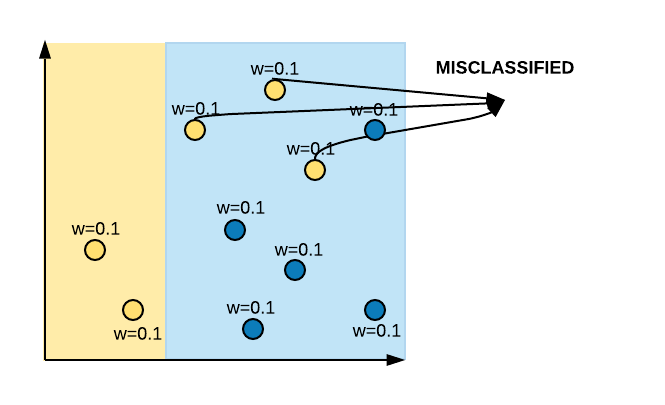
\includegraphics[width = \textwidth]{../assets/ensemble/diagrams/ada_iter1_misclassify}
									\vspace{-20pt}
					\caption{$\alpha_1=0.42$}
				\end{figure}
				
			\end{column}
			
			
			\pause \begin{column}{0.4\textwidth}
				\centering
				\begin{figure}
					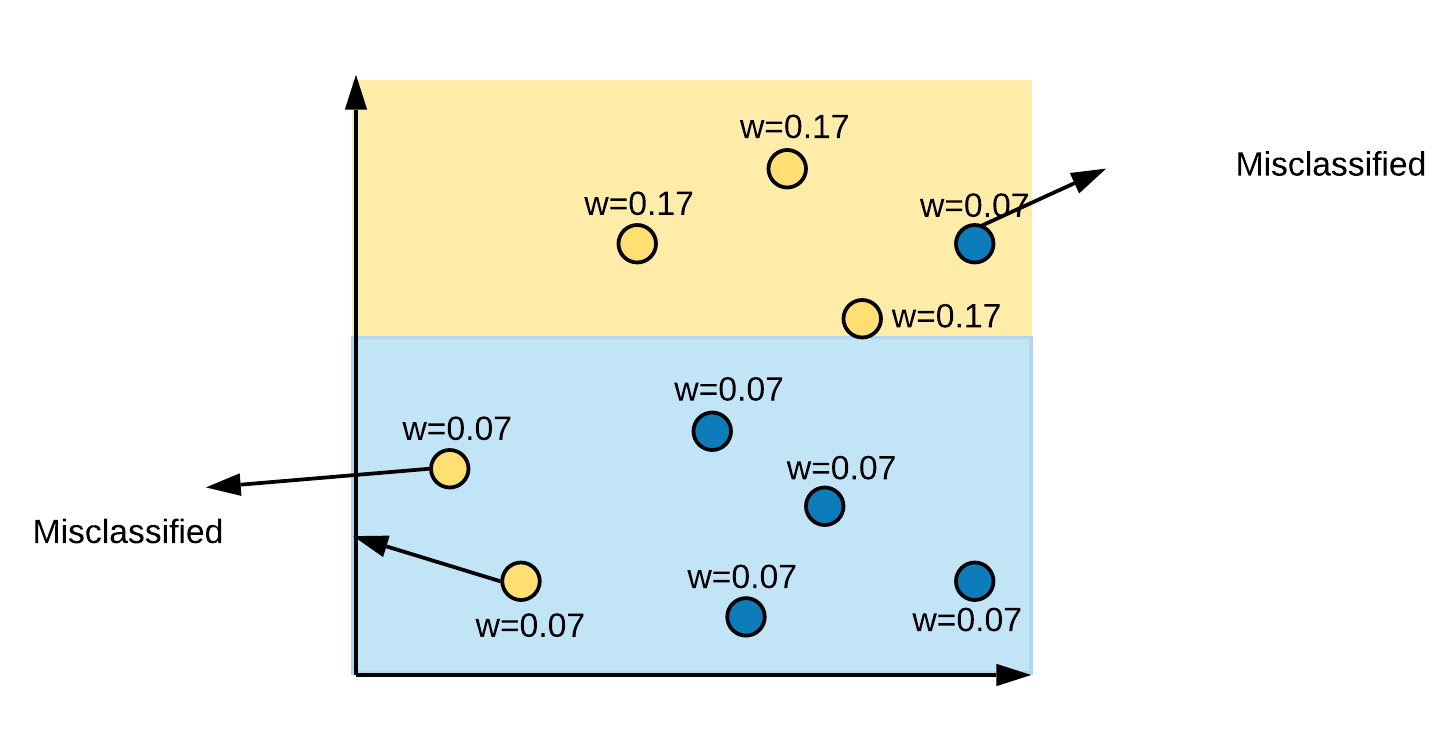
\includegraphics[width = \textwidth]{../assets/ensemble/diagrams/ada_iter2_misclassify}
					\vspace{-20pt}
					\caption{$\alpha_2=0.66$}
				\end{figure}
	
			\pause \end{column}
					\begin{column}{0.3\textwidth}
				\centering
				\begin{figure}
					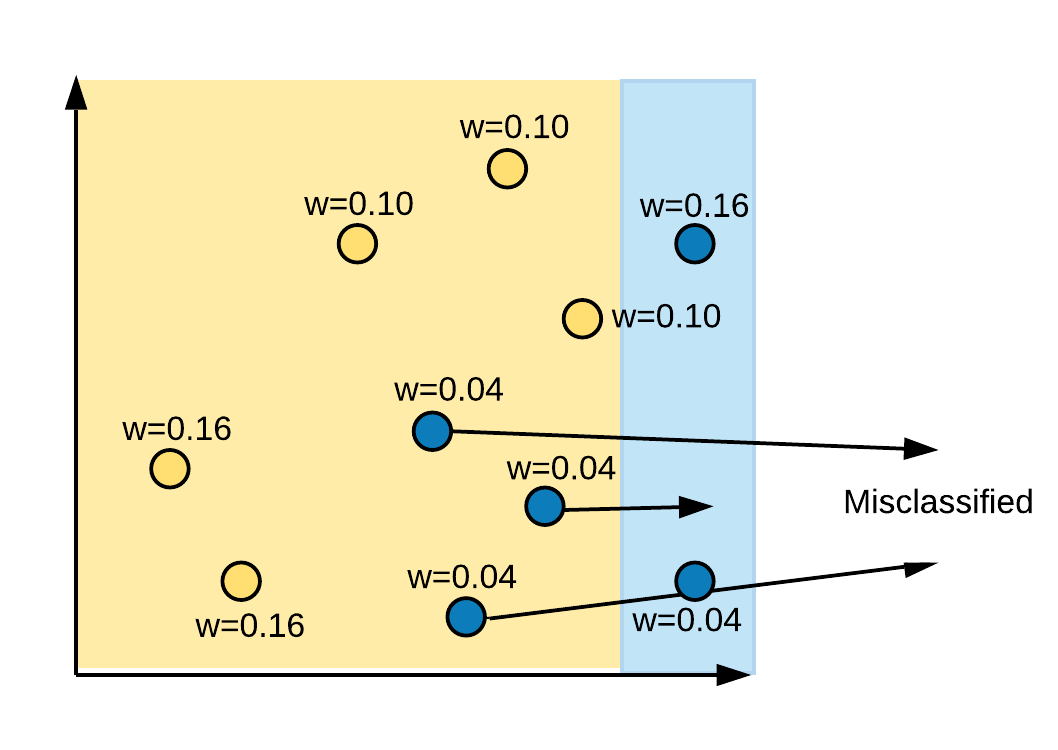
\includegraphics[width = \textwidth]{../assets/ensemble/diagrams/ada_iter3_misclassify}
									\vspace{-20pt}
					\caption{$\alpha_3=0.99$}
				\end{figure}
				
			\end{column}
		\end{columns}
	
		\begin{columns}
			\pause \begin{column}{0.5\textwidth}
				\begin{figure}
				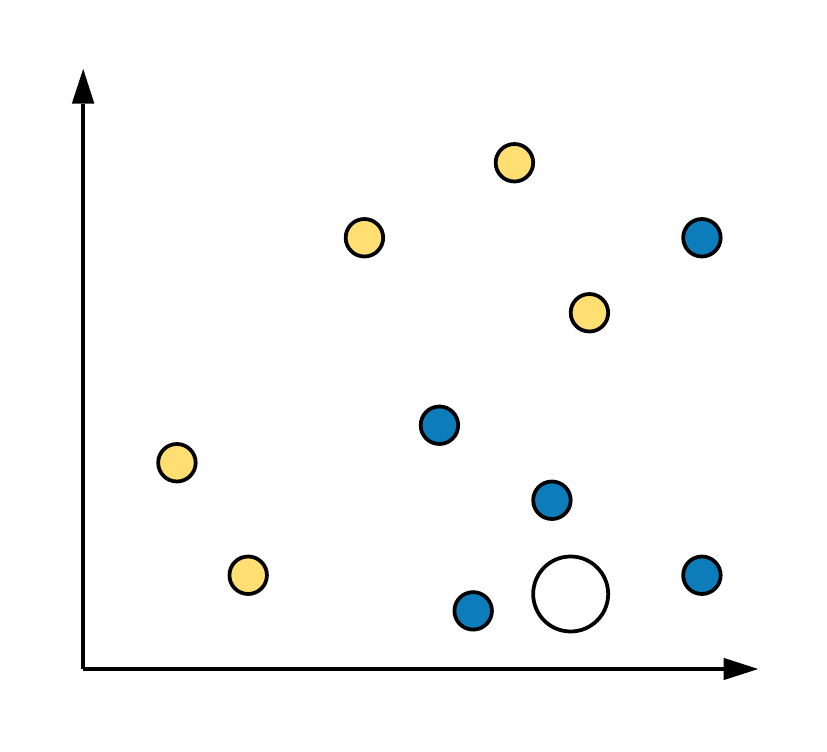
\includegraphics[scale=0.1]{../assets/ensemble/diagrams/testing}
				\end{figure}
			\end{column}
		
		\begin{column}{0.5\textwidth}
			\pause Let us say, yellow class is +1 and blue class is -1
			
			\pause Prediction = SIGN(0.42*-1 + 0.66*-1 + 0.99*+1) = Negative = blue
		\end{column}
		\end{columns}
	
\end{frame}

% \begin{frame}

%     \pause \begin{column}{0.4\textwidth}
%       \centering
%       \begin{figure}
%         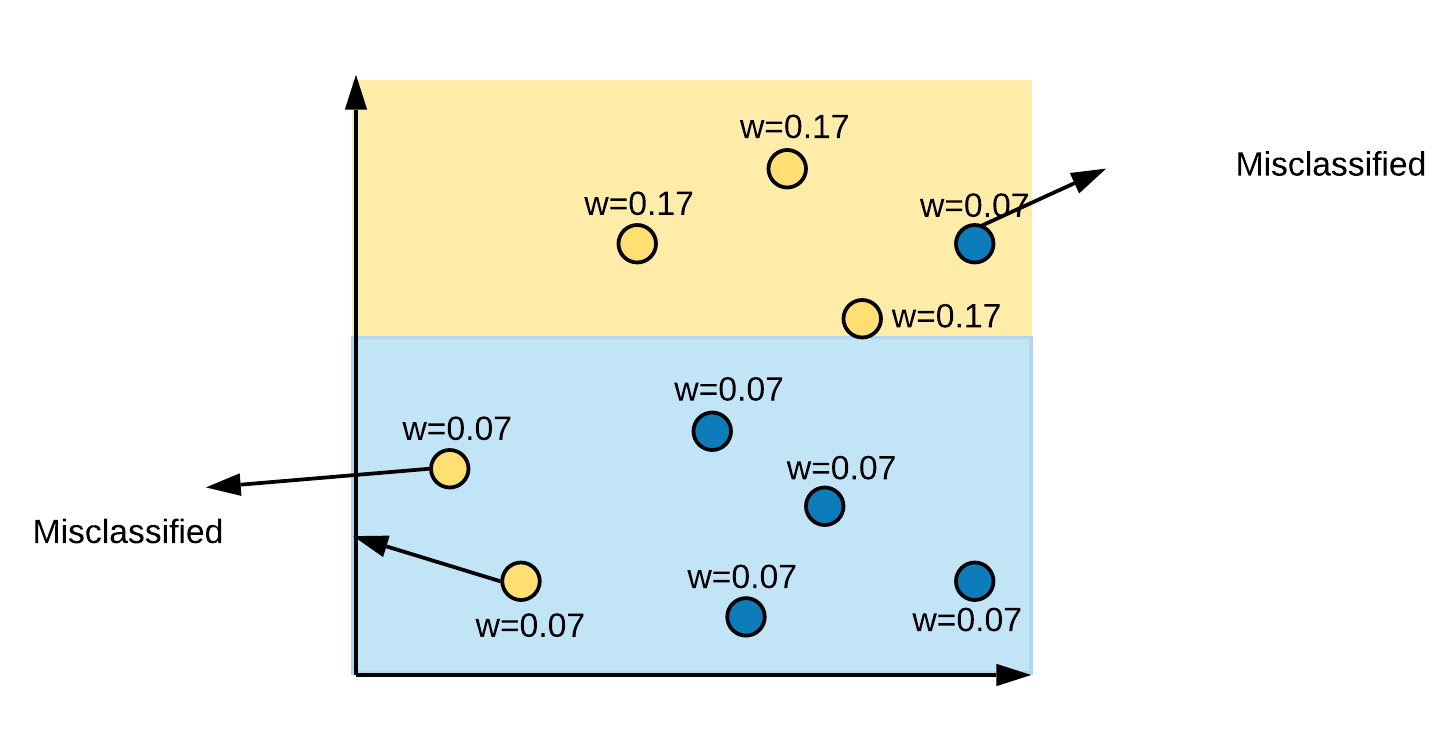
\includegraphics[width = \textwidth]{../assets/ensemble/diagrams/ada_iter2_misclassify}
%         \vspace{-20pt}
%         \caption{$\alpha_2=0.66$}
%       \end{figure}
% 	\end{column}
% \end{columns}

% \end{frame}
		
% 	\begin{frame}
%       \pause \end{column}
%     \begin{column}{0.3\textwidth}
%       \centering
%       \begin{figure}
%         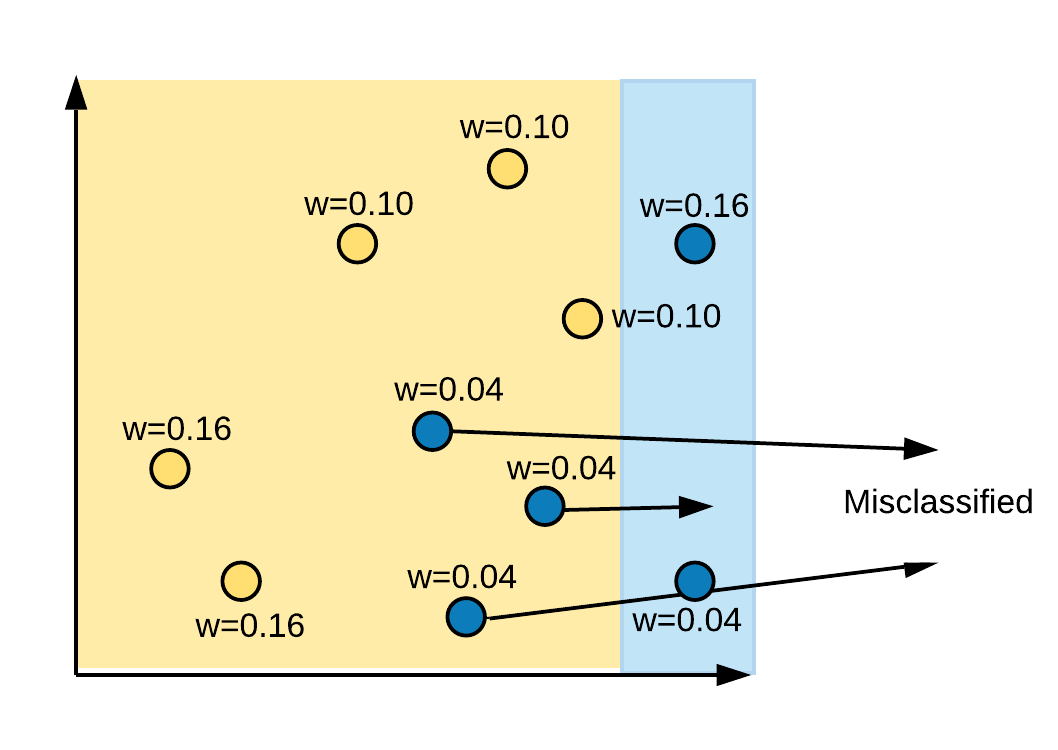
\includegraphics[width = \textwidth]{../assets/ensemble/diagrams/ada_iter3_misclassify}
%         \vspace{-20pt}
%         \caption{$\alpha_3=0.99$}
%       \end{figure}

%     \end{column}
%   \end{columns}

%   \begin{columns}
%     \pause \begin{column}{0.5\textwidth}
%       \begin{figure}
%         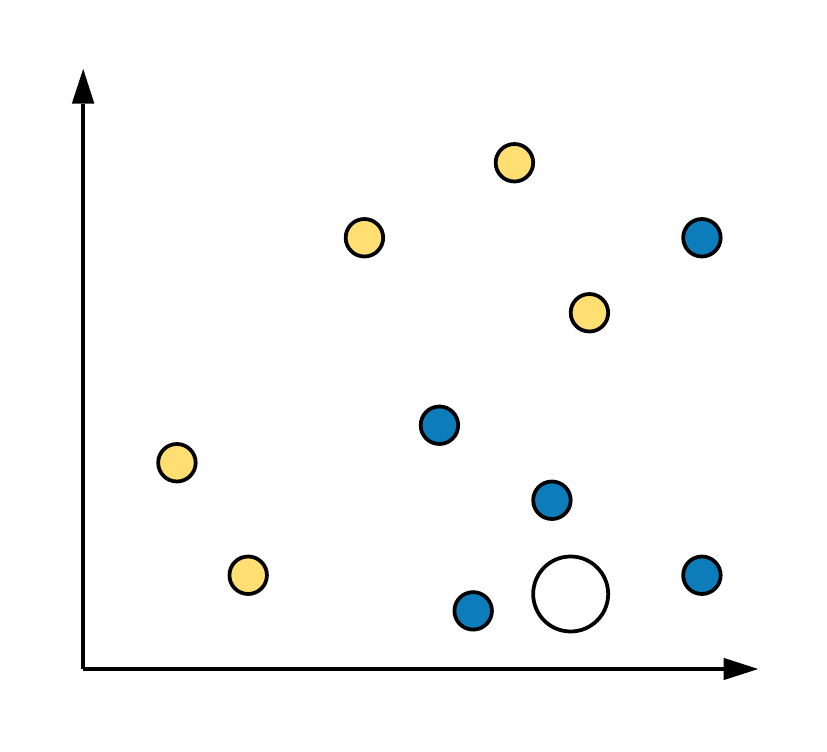
\includegraphics[scale=0.1]{../assets/ensemble/diagrams/testing}
%       \end{figure}
%     \end{column}

%     \begin{column}{0.5\textwidth}
%       \pause Let us say, yellow class is +1 and blue class is -1

%       \pause Prediction = SIGN(0.42*-1 + 0.66*-1 + 0.99*+1) = Negative = blue
%     \end{column}
%   \end{columns}

% \end{frame}


\begin{frame}{Intuition behind weight update formula}
  \begin{columns}
    \pause \begin{column}{0.5\textwidth}

      \begin{figure}[htp]
        \centering
        \begin{notebookbox}{https://nipunbatra.github.io/ml-teaching/notebooks/boosting-explanation.html}
          % 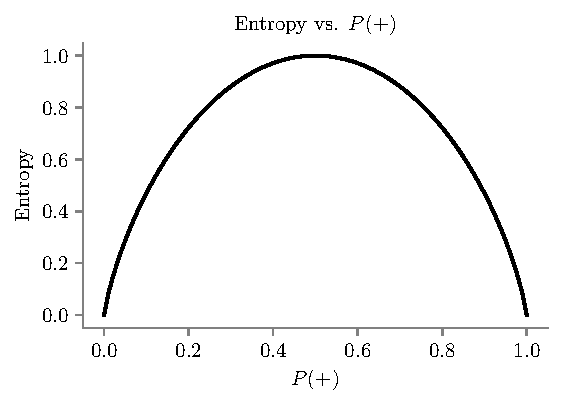
\includegraphics[scale=0.8]{../figures/decision-trees/entropy.pdf}
          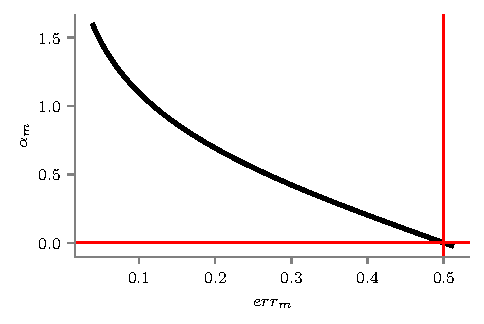
\includegraphics[scale=0.55]{../assets/ensemble/figures/alpha-boosting.pdf}
        \end{notebookbox}
      \end{figure}
    \end{column}
    \pause \begin{column}{0.5\textwidth}
      \begin{figure}[htp]
        \centering
        \begin{notebookbox}{https://nipunbatra.github.io/ml-teaching/notebooks/boosting-explanation.html}
          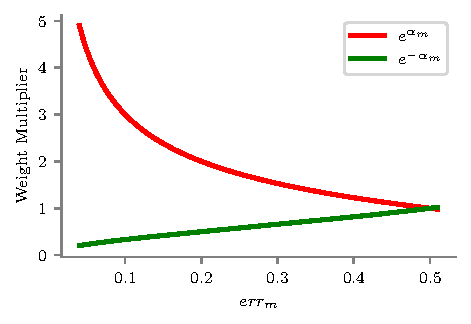
\includegraphics[scale=0.55]{../assets/ensemble/figures/alpha-boosting-weight.pdf}
        \end{notebookbox}
      \end{figure}
    \end{column}
  \end{columns}


\end{frame}

\begin{frame}{ADABoost for regresion}
  From Paper: Improving Regressors using Boosting Techniques

  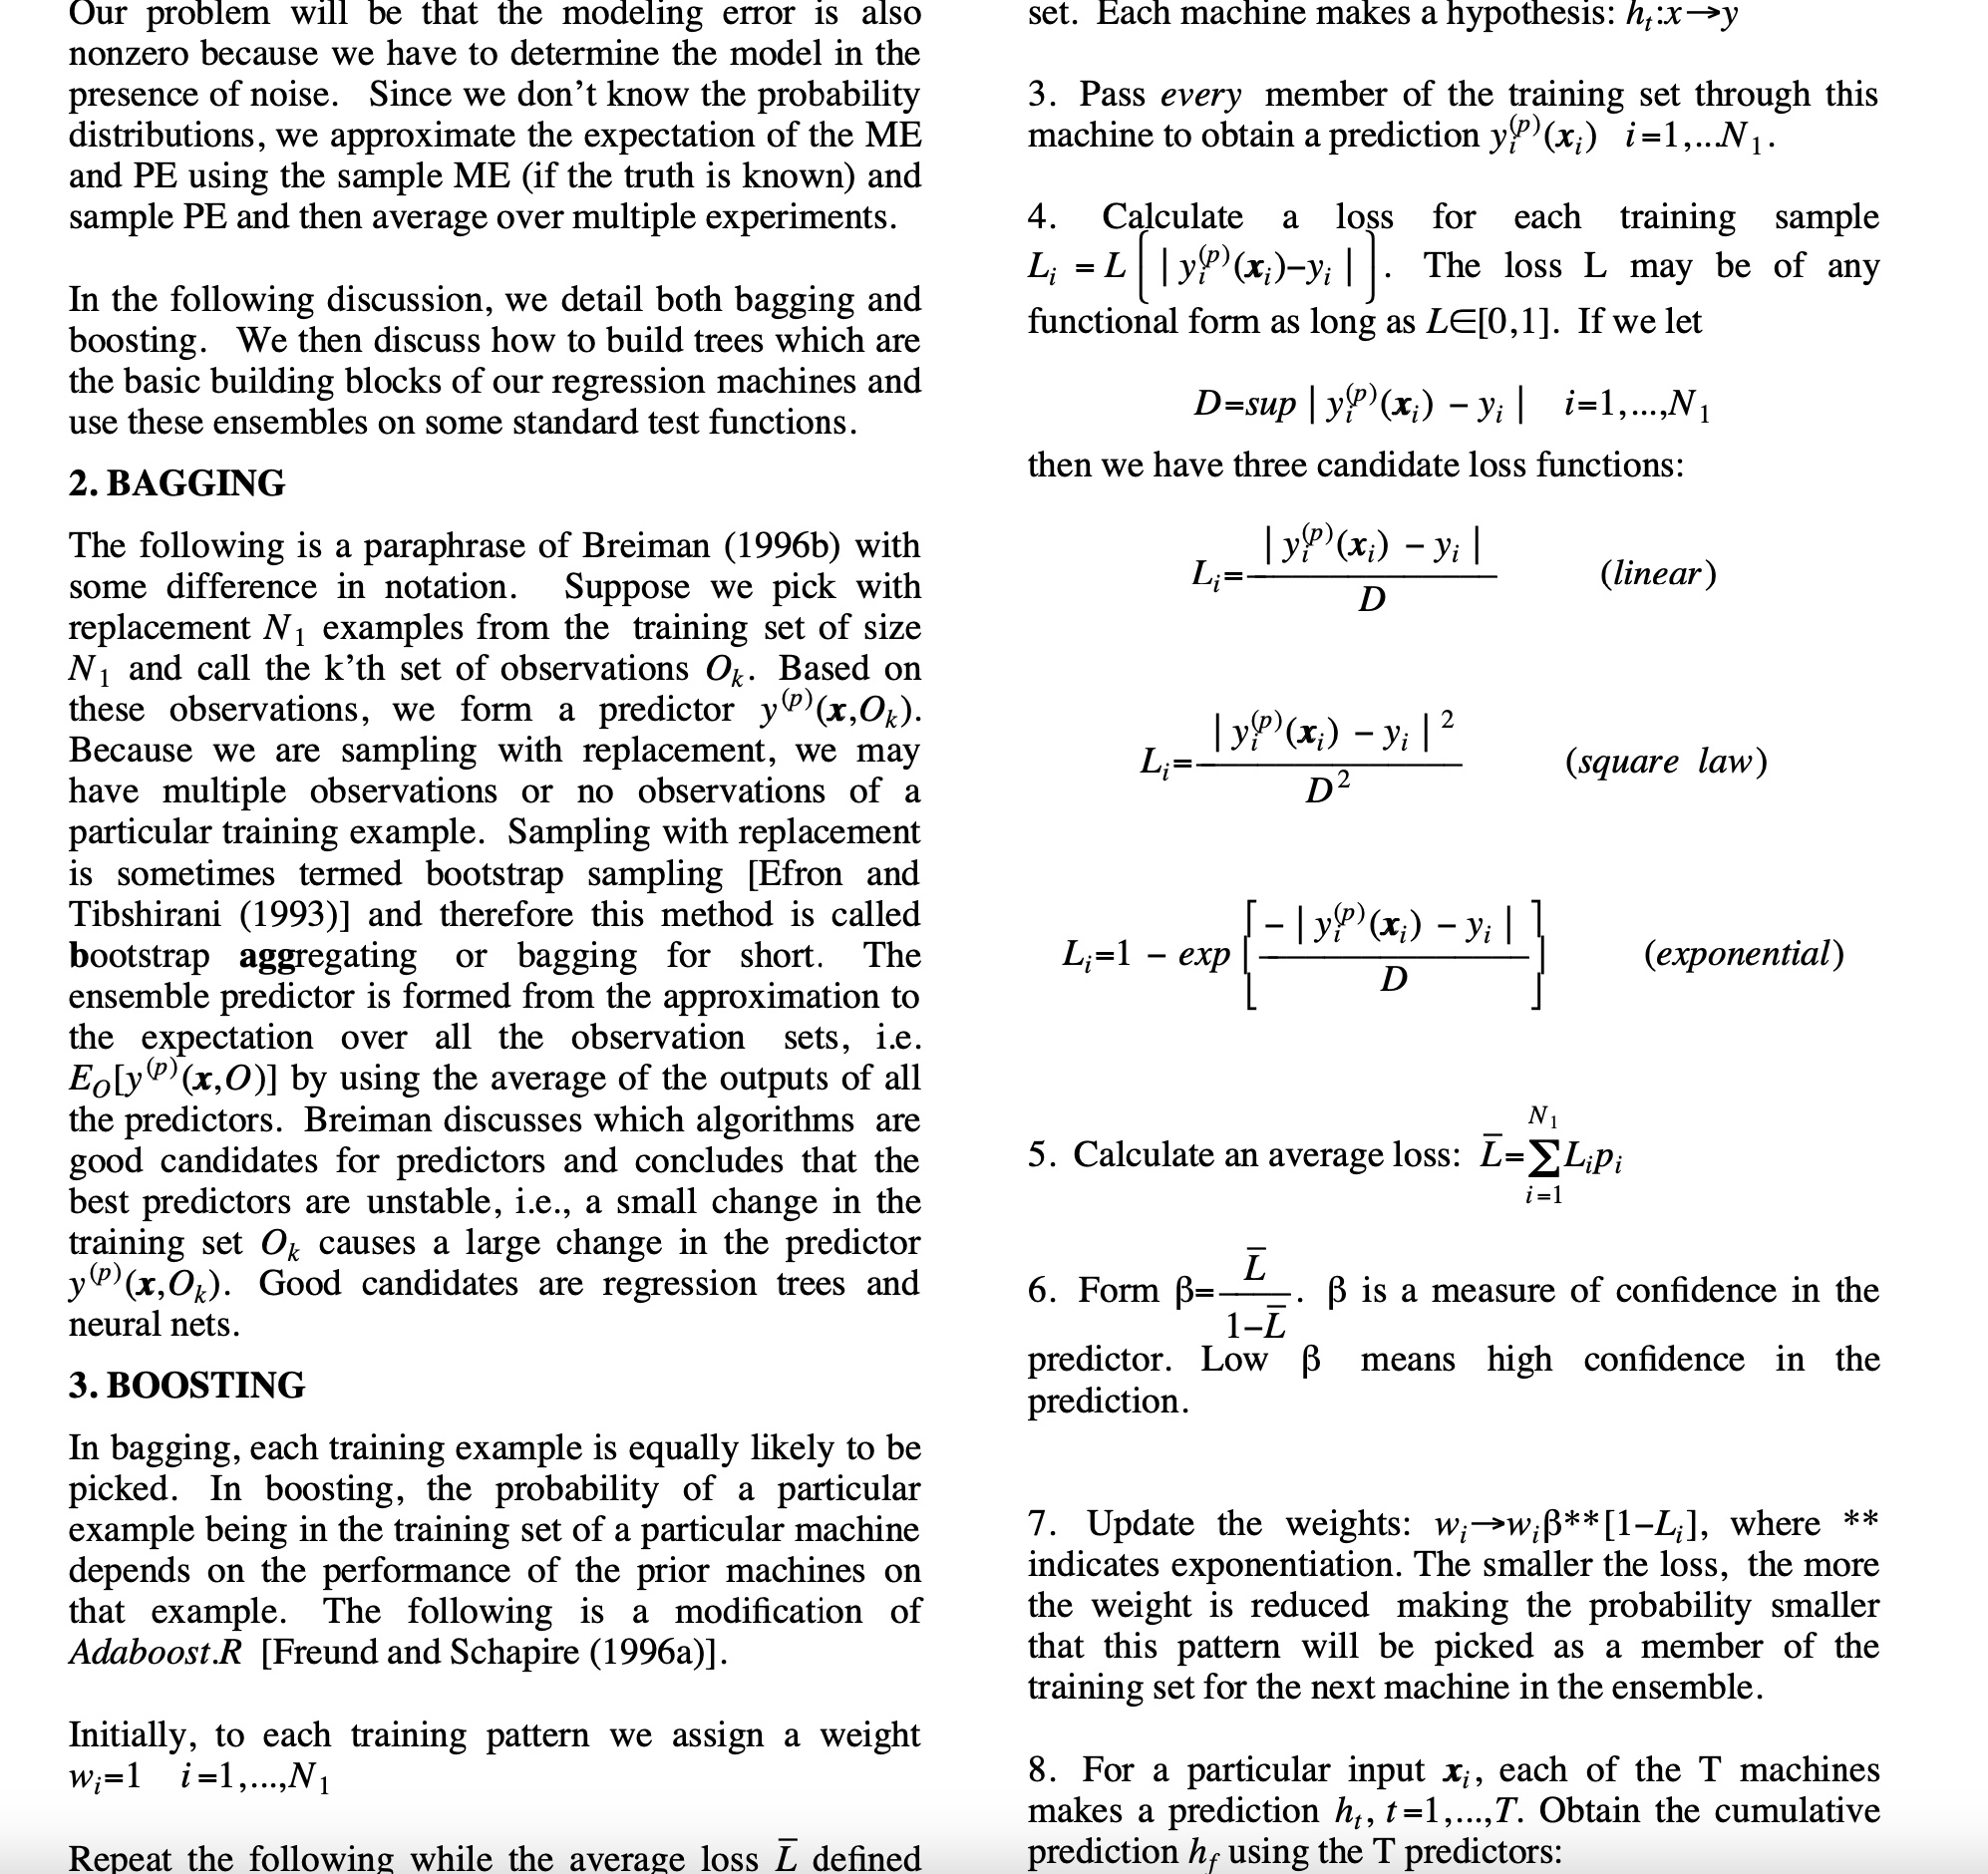
\includegraphics[scale=0.1]{../assets/ensemble/diagrams/adaboost-regression.jpg}
  
\end{frame}

\begin{frame}{Random Forest}
  \begin{itemize}
    \item Random Forest is an ensemble of decision trees.
    \item We have two types of bagging: bootstrap (on data) and random subspace (of features).
    \item As features are randomly selected, we learn decorrelated trees and helps in reducing variance.
  \end{itemize}
\end{frame}

\begin{frame}{Random Forest}
There are 3 parameters while training a random forest number of trees, number of features (m), maximum depth.\\
\vspace{1cm}
\underline{Training Algorithm}\\
\begin{itemize}
	\item For $i^{th}$ tree ($i \in \{1 \cdots N\}$), select $n$ samples from total $N$ samples with replacement.\\
%   \item for $tree$ in $1, \dots,$ $number$ $of$ $trees$ $\]$
		
		\item Learn Decision Tree on selected samples for $i^{th}$ round.
		 

\end{itemize}

\underline{Learning Decision Tree (for RF)}\\
\begin{itemize}
	\item For each split, select $m$ features from total available $M$ features and train a decision tree on selected features
\end{itemize}


\end{frame}

\begin{frame}{Dataset }
  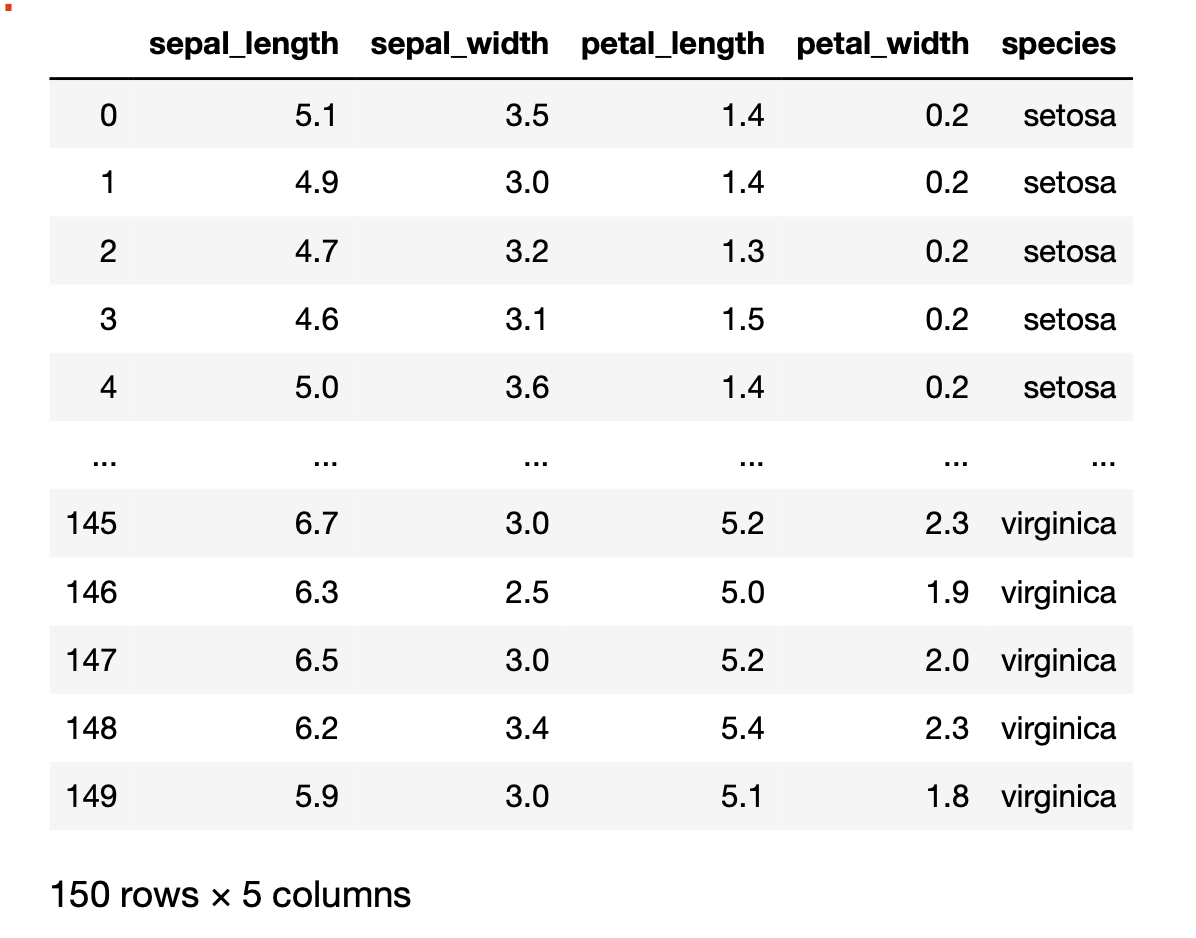
\includegraphics[scale=0.5]{../assets/ensemble/diagrams/dataset-iris.png}
\end{frame}


% \begin{frame}{Random Forest}
% There are 3 parameters while training a random forest ``$number$ $of$ $trees$'', ``$number$ $of$ $features'' (m)$, ``$maximum$ $depth$''.\\
% \vspace{1cm}
% \underline{Training Algorithm}\\
% \begin{itemize}
%   \item for $depth$ in $[1, \dots,$ $maximum$ $depth$ $]$
%     \begin{itemize}
%       \item for $tree$ in $[1, \dots,$ $number$ $of$ $trees$ $]$
%       \begin{itemize}
%         \item For each split, select ``$m$'' features from total available $M$ features and train a decision tree on selected features
%         
%       \end{itemize}
%     \end{itemize}
% \end{itemize}
% \end{frame}



\newcounter{tree}
\forloop{tree}{0}{\value{tree} < 10}{
  \begin{frame}{Decision Tree \# \thetree}
    \begin{figure}
      % \includegraphics[scale=0.25]{../assets/ensemble/figures/feature-imp-\thetree.pdf}
      \centering
      \begin{notebookbox}{https://nipunbatra.github.io/ml-teaching/notebooks/ensemble-feature-importance.html}
        \includegraphics[scale=0.25]{../assets/ensemble/figures/feature-imp-\thetree.pdf}
        
      \end{notebookbox}
    \end{figure}
  \end{frame}
}


\begin{frame}{Feature Importance\footnotemark}
  \begin{figure}
    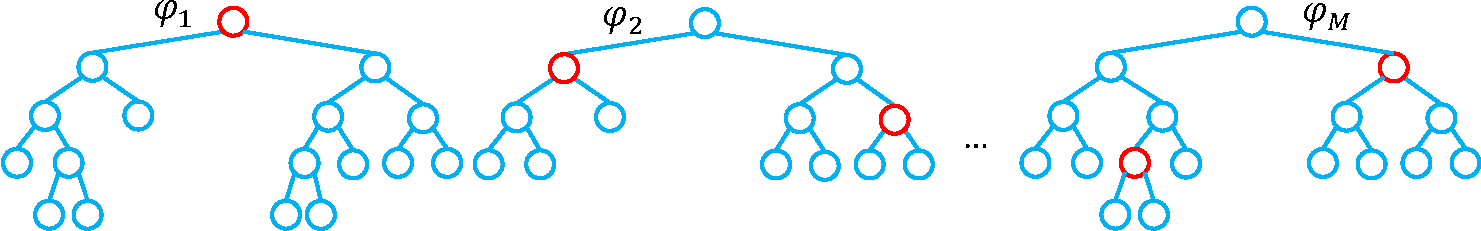
\includegraphics[scale=0.4]{../assets/ensemble/diagrams/mdi.pdf}
  \end{figure}
  Importance of variable $X_j$ for an ensemble of $M$ trees $\varphi_{m}$ is:
  \begin{equation*}
    \text{Imp}(X_j) = \frac{1}{M} \sum_{m=1}^M \sum_{t \in \varphi_{m}} 1(j_t = j) \Big[ p(t) \Delta i(t) \Big],
  \end{equation*}
  where $j_t$ denotes the variable used at node $t$, $p(t)=N_t/N$ and $\Delta i(t)$ is the impurity reduction at node $t$:
  \begin{equation*}
    \Delta i(t) = i(t) - \frac{N_{t_L}}{N_t} i(t_L) - \frac{N_{t_r}}{N_t} i(t_R)
  \end{equation*}
  \footnotetext[1]{Slide Courtesy Gilles Louppe}

\end{frame}


\begin{frame}{Computed Feature Importance}
  \begin{figure}[htp]
    \centering
    \begin{notebookbox}{https://nipunbatra.github.io/ml-teaching/notebooks/ensemble-feature-importance.html}
      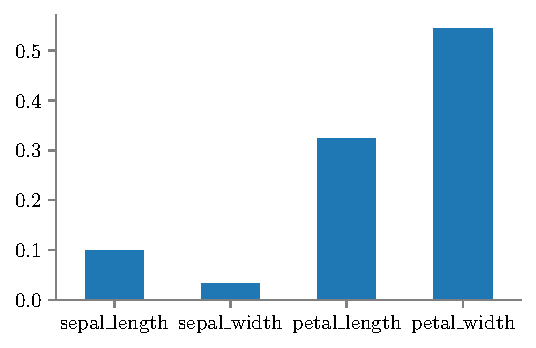
\includegraphics[scale=0.8]{../assets/ensemble/figures/feature-imp-forest.pdf}
    \end{notebookbox}
\end{figure}
  % 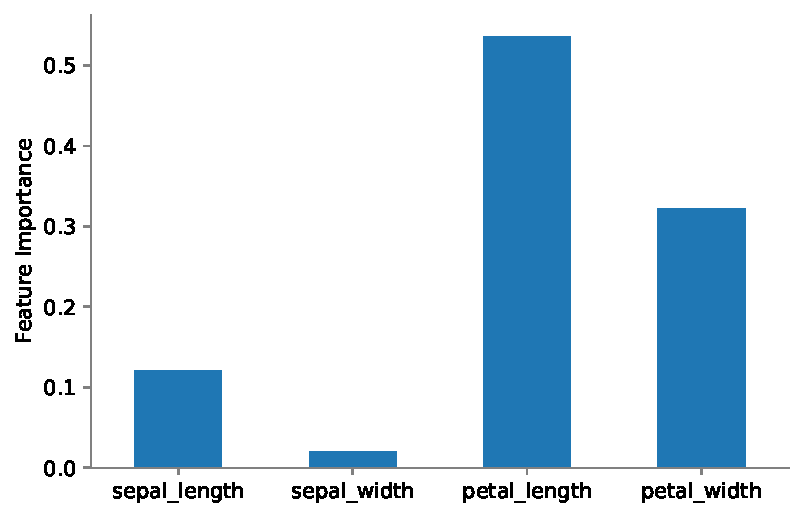
\includegraphics[scale=0.6]{feature-importance.pdf}
\end{frame}

\end{document}
